\documentclass[12pt]{article}
\usepackage[margin = 1in]{geometry}
\usepackage[USenglish]{babel}
\usepackage{natbib}
\usepackage{multirow}
\usepackage{graphicx, subfigure}
\usepackage{fancyhdr}
\usepackage{setspace}
\usepackage{verbatim}
\usepackage{booktabs}
\usepackage{amsmath}
\usepackage{lscape}
\usepackage{dcolumn}
\usepackage{floatrow}
\usepackage[title]{appendix}
\usepackage{xcolor}
\usepackage{todonotes}
\usepackage{titletoc}
\usepackage[colorlinks=true,citecolor=red!50!black,urlcolor=blue!50!black,linkcolor=red!50!black]{hyperref}

\author{Patrick W. Kraft\footnote{Ph.D. Student, Stony Brook University, \href{mailto:patrick.kraft@stonybrook.edu}{patrick.kraft@stonybrook.edu}.
%I thank Jennifer Jerit, Stanley Feldman, Scott Clifford, Peter DeScioli, Jason Barabas, and participants of the Political Science Graduate Student Colloquium at Stony Brook University as well as participants at the panel of the 2015 Annual Meeting of the Midwest Political Science Association for helpful comments on earlier versions of this manuscript.
}}
\date{today}

\title{Moral Foundations of Political Reasoning\footnote{An earlier version of this paper was presented at the 73rd Annual Conference of the Midwest Political Science Association, April 16-19, 2015. The manuscript and code are available on GitHub: \url{https://github.com/pwkraft/mft}.}\\
\large{Investigating the Moral Underpinnings of Political Judgment}}
\date{\today}


\begin{document}
\maketitle
\onehalfspacing

\begin{abstract}
This paper investigates how differences in moral judgments between liberals and conservatives shape and structure political reasoning. Using the open-ended survey responses in the 2008 and 2012 American National Election Study, I utilize moral word lists to identify references to basic moral intuitions when individuals report on their attitudes towards political parties and candidates. The results show that liberals and conservatives rely on different sets of moral foundations when evaluating political actors. Furthermore, the emphasis on specific moral considerations in political evaluations predicts political participation, attitudes towards parties and candidates, as well as voting behavior, even after controlling for party identification. However, ideological differences in moral reasoning appear to be context-specific and are not always consistent with theoretical expectations of Moral Foundations Theory.

%\vspace{\baselineskip}
%\noindent \textbf{Keywords:} Moral Foundations Theory, Political Reasoning, Ideology, Political Behavior, Open-ended Survey Responses
\end{abstract}
\newpage


\section{Introduction}

Political discussions often revolve around underlying moral issues. Notable contemporary examples include debates about stem cell research, abortion, and same-sex marriage \citep[e.g.][]{koleva2012tracing,clifford2015concerns}. Even issues that are not necessarily considered as intrinsically ``moral'', such as those related to the economy, can indeed be connected to underlying moral convictions \citep{ryan2014reconsidering}. Moral values therefore serve as a potential source for coherence in political attitudes and thereby shape individual belief systems. According to one prominent theoretical approach, \textit{Moral Foundations Theory}, moral thinking is organized by five central ``foundations'': harm/care, fairness/reciprocity, ingroup/loyalty, authority/respect, and purity/sanctity \citep{haidt2008moral}. Liberals and conservatives differ in their relative emphasis of these foundations, with liberals prioritizing the foundations of harm/care and fairness/reciprocity, and conservatives endorsing all five foundations more or less equally \citep{graham2009liberals}. A growing body of work has documented the political relevance of moral foundations in the area of vote choice \citep{iyer2010beyond, franks2015using}, political attitudes and issue preferences \citep{koleva2012tracing, low2015moral, clifford2015concerns}, and candidate trait evaluations \citep{clifford2014linking}.

Yet, nearly all existing work relies on the Moral Foundations Questionnaire (MFQ) as a measure of moral reasoning \citep[but see][]{clifford2014linking}. The MFQ consists of a series of items that explicitly ask people to rate the relevance of different considerations when making decisions about right and wrong.\footnote{E.g. ``Whether or not some people were treated differently than others'' as an indicator for the fairness/reciprocity dimension (c.f. \url{http://www.moralfoundations.org/}).} The questionnaire also asks individuals to indicate their level of agreement with statements that represent the values implied by the five foundations.\footnote{E.g. ``I am proud of my country’s history'' as an indicator for the ingroup/loyalty dimension.} Some have criticized the MFQ because it does not ask people to make moral judgments per se. Indeed, \citet[1031]{graham2009liberals} describe the reports on moral relevance as ``self-theories of moral judgment,'' rather than direct measures of judgment itself. Such abstract self-theories might, in turn, deviate from actual judgments in specific situations \citep[see][for an alternative way to measure moral judgment]{clifford2015moral}.

The present study raises a more fundamental point about the ability of the MFQ to measure moral reasoning. While the past research shows differences between liberals and conservatives in terms of their latent emphasis on moral foundations, it remains an open question whether people utilize the foundations in their day-to-day political reasoning--i.e., without being prompted by the language of a questionnaire. By directly asking people about the importance of considerations related to the five foundations, the MFQ presupposes an important link that requires more careful empirical investigation. This study examines whether differences in moral reasoning between liberals and conservatives manifest themselves in a more unobtrusive context (i.e., without explicitly asking people to think about morality as is done on the MFQ). Using data from the 2008 and 2012 American National Election Study, I code the responses to the open-ended likes-dislikes questions according to the moral word lists introduced by \citet{graham2009liberals}. Finding similar patterns in this context would provide stronger evidence for the claim that political reasoning is influenced by basic moral intuitions. 

Overall, the results indicate that liberals and conservatives differ in their reliance on specific moral considerations--even without being cued to think about morality. Furthermore, moral reasoning powerfully influences political participation, candidate evaluation, and voting behavior, even after controlling for individual party identification. While the ideological differences are broadly consistent with Moral Foundations Theory, moral reasoning in the realm of politics is more context-specific than previous research suggests. From a methodological standpoint, the research presented here illustrates the usefulness of open-ended survey measures for examining the antecedents of political reasoning.


\section{Theoretical Framework}

To what extent are political belief systems and ideologies shaped, structured, and constrained by individual psychological characteristics and underlying motivations? This question has been of frequent scholarly interest in political science and related disciplines, yielding a wide array of different perspectives. Early accounts emphasized how ordinary citizens lack consistent political attitudes and knowledge necessary to form meaningful ideologies in the first place \citep[e.g.][]{converse1964nature}. Other scholars argued, that there are few differences between liberal and conservative attitudes, that ideology has no strong behavioral impacts, or that psychological mechanisms do not differ between liberals and conservatives \citep[see][for an overview regarding each of these points]{jost2006end}.

However, with increasing levels of polarization and partisan sorting in contemporary politics \citep[e.g.][]{iyengar2015fear}, the study of ideology recently gained renewed attention and relevance, a development that was termed as the ``End of the End of Ideology'' by John T. Jost \citeyearpar{jost2006end}. It is therefore no surprise that there has been a surge in research investigating basic underpinnings of ideology \citep[see also][]{jost2003political,jost2009political}. For example, it has been shown that liberals and conservatives differ with regard to personality characteristics \citep{gerber2010personality,hirsh2010compassionate,de2015personality,feldman2014understanding}, social values \citep{schwartz2010basic,schwartz2011basic,piurko2011basic}, or more fundamental factors such as disgust sensitivity \citep{inbar2009conservatives} or mortality salience \citep{burke2013death}.

Another potential source for structure and constraint in political ideology that is frequently discussed in the literature focuses on moral values as determinants of political attitudes and preferences \citep{lakoff1995metaphor,haidt2008moral,mcadams2008family}. The following section will discuss this strand of research in more detail.


\subsection{Moral Foundations Theory}

In one of his influential earlier works on moral psychology, \citet{haidt2001emotional} argued that moral judgment is not based on rational reasoning but rather on automatic and affective intuitions, which are in turn influenced by social and environmental factors. More specifically, \citet[825]{haidt2001emotional} argues that moral intuition ``appears to be the automatic output of an underlying, largely unconscious set of interlinked moral concepts. These concepts may have some innate basis [...], which is then built up largely by metaphorical extensions from physical experience.'' According to this view, explicit moral reasoning is better described as a rationalization of these intuitions, which are partially innate and therefore ``organized, to some extent, in advance of experience'' (\citealt[367]{haidt2008moral}, but see \citealt{suhler2011can}).

\citet{haidt2008moral} identified five basic intuitions which build the psychological foundations of human morality and are inherently linked to evolutionary adaptive challenges that appear cross-culturally. These five basic intuitions are \textit{Harm/Care}, \textit{Fairness/Reciprocity}, \textit{Ingroup/Loyalty}, \textit{Authority/Respect}, and \textit{Purity/Sanctity} \citep[see also][]{graham2011mapping}.\footnote{Subsequent accounts of Moral Foundations Theory discussed the inclusion of further dimensions, such as \textit{Liberty/Oppression} \citep[c.f.][]{graham2013moral,haidt2012righteous}. However, the analyses presented here will only focus on the dimensions initially suggested in \citet{haidt2008moral}.} They represent an innate draft of morality that is further edited by individual experience. This editing process, in turn, is determined by the development of moral virtues as personal characteristics as well as moral narratives \citep{haidt2008moral}.


\subsection{Moral Values and Political Ideology}

Moral and social values have been discussed as one of the underlying personality characteristics that determine broader political beliefs. For example, \citet{piurko2011basic} described how basic personal values structured underlying motivational meanings of liberal and conservative political orientations \citep[see also][]{schwartz2010basic,schwartz2011basic}. Focusing more closely on moral values, \citet{lakoff1995metaphor} argued that conservative and liberal belief systems can be differentiated by their relative emphasis on specific moral metaphors, namely the strict father model as well as the nurturant parent model. In a subsequent study, \citet{barker2006competing} showed that these nurturant and disciplinarian visions of parental roles can indeed be connected to ideologically coherent views.

The possible connection between moral values and political belief systems also became a major focus in the context of the Moral Foundations framework \citep[c.f.][]{haidt2012righteous}. \citet{haidt2007morality} as well as \citet{graham2009liberals} argued that liberal morals focus on individualizing foundations, which include harm/care and fairness/reciprocity. Conservatives, on the other hand, also emphasize the remaining foundations of ingroup/loyalty, authority/respect, and purity/sanctity, which are labeled as binding foundations. One notable aspect about their expectations as well as their empirical results is that conservatives do not prioritize the individualizing foundations less than liberals. They rather endorse all five foundations more equally and therefore emphasize the binding foundations more than liberals.

\citet{graham2009liberals} demonstrated in their analyses that liberals showed greater endorsement and use of harm/care and fairness/reciprocity foundations when they were asked to evaluate the relevance of moral concerns, when they made explicit moral judgments, as well as in the context of moral trade-offs. Throughout these studies, conservatives endorsed and used the five foundations more equally. The final study presented by \citet{graham2009liberals} consisted of a quantitative analysis of sermons from liberal and conservative churches. The authors proposed a dictionary of words (and word stems) that signal references to the specific moral foundations and showed that liberal sermons were more likely to contain expressions that can be ascribed to the moral foundations of harm/care and fairness/reciprocity. As will be further described below, the analyses presented here will utilize the same dictionary in order to assess moral references in the context of open-ended survey responses.

Subsequent studies extended the initial findings, for example by examining the the relationship between moral intuitions and multi-dimensional conceptualizations of ideology \citep[c.f.][]{haidt2009above}.  Other scholars showed that moral concerns predicted attitudes towards a wide variety of divisive political issues \citep[e.g.][]{koleva2012tracing,low2015moral}. \citet{federico2013mapping} linked moral foundations to individual social dominance orientation (SDO) and right-wing authoritarianism (RWA). Further research directly investigated the relationship between moral foundations and candidate preferences \citep{iyer2010beyond} or trait inferences about candidates \citep{clifford2014linking}. Moral foundations have also been shown to predict turnout \citep{johnson2014ideology} as well as voting behavior in the 2012 US Presidential election \citep{franks2015using}.
%more details on these studies maybe


\subsection{Sophistication and the `Missing Link' to Political Reasoning}

Overall, the studies discussed so far strongly support the view that the underlying moral intuitions conceptualized in the Moral Foundations framework differ systematically between liberals and conservatives and are linked to political attitudes, evaluations, as well as behavior. However, most of these studies relied on the MFQ and related measures, which do not allow us to directly examine the conditions under which the connection between moral values and political ideology manifests itself when citizens reason about politics and evaluate political actors. Indeed, \citet{haidt2008moral} emphasized the importance of moral narratives in the development of moral thinking and \citet{mcadams2008family} demonstrated how conservatives and liberals differed in terms of moral references in life-narrative interviews. Other research discussed above showed correlational evidence linking moral foundations as measured by the MFQ to different political outcomes. But do the implicit moral narratives actually shape citizens' political reasoning in the way the previous studies suggest?

From a theoretical perspective, moral foundations are often viewed as stable predispositions or personality characteristics that affect attitudes and preferences regardless of potential individual moderators and contextual effects. However, moral reasoning understood as the actual incorporation of moral considerations in a specific political context could be much more variable. There are some studies that indicated that many individuals make frequent references to values when discussing their policy preferences \citep{feldman1992political} and that the reliance on basic values is not contingent on individual characteristics such as political sophistication \citep[e.g.][]{goren2001core,goren2004political,marietta2007values}. However, other studies in the domain of moral foundations suggested that campaigns and elite communication can have important influences on individual moral reasoning. For example, \citet{clifford2013words} argued that on the elite level, proponents and opponents of stem cell research place distinctive weights on moral foundations which in turn affected the public attitudes and the underlying considerations related to the issue. A subsequent study showed that elite rhetoric plays an important role in linking individual moral foundations with political attitudes \citep{clifford2015concerns}. \citet{day2014shifting} presented further evidence indicating that issue framing in terms of moral foundations changes individual attitudes. While these studies do not contradict Moral Foundations theory as such, they do cast some doubt on the notion that moral reasoning in politics should be considered as a pure reflection of stable moral intuitions. Quite contrary, individuals who are more exposed to the political process and resulting elite communications might be more likely to incorporate moral considerations in their political reasoning. Individuals who are not engaged in politics, on the other hand, might focus on other characteristics than morality when thinking about and forming their political preferences. These differences could not be investigated by relying solely on MFQ and related measures to conceptualize moral reasoning. Instead, it is necessary to differentiate between moral \textit{foundations} as stable predispositions and personality characteristics, and moral \textit{reasoning} as the actual reliance on specific moral considerations and arguments, both from a theoretical as well as a measurement perspective. Previous research largely neglected this difference.

In the present paper, it is therefore argued that the extent to which individuals rely on moral considerations when evaluating political actors is not necessarily stable among individuals and across contexts. Rather, the tendency to emphasize moral foundations is contingent upon individual levels of political sophistication, media exposure, and political discussions. Moral Foundations Theory proposes that innate differences in the emphasis of moral considerations provide the basis for diversity in ideological and political reasoning. However, moral reasoning can also be viewed as a rhetorical tool that citizens use in order to support their preferences and bolster their views in front of others. If the emphasis on moral considerations is indeed contingent upon political engagement, exposure to political media, and frequent discussions, moral reasoning should be viewed as the product of a learning process in the political environment.
% I think this part needs more details and a through revision...
% more MFQ measuremnt critique maybe?


\section{Empirical Analyses}

\subsection{Overview and Hypotheses}

The first step of the analyses presented here will be to replicate the findings connecting moral foundations as measured by the MFQ and ideology using open-ended survey responses. Insofar as moral intuitions play an important role in elite-level discourse, citizens may rely on the moral foundations when reporting their attitudes towards political actors, even if they are not explicitly asked to do so. As such, the first hypothesis can be stated as follows:

\vspace{0.3cm}
\begin{tabular}{lp{12cm}}
\textsl{Hypothesis 1:} & Liberals are more likely to emphasize moral foundations of harm/care and fairness/reciprocity  than conservatives when evaluating political parties and candidates in the context of open-ended survey items. On the other hand, conservatives are more likely to emphasize moral foundations of ingroup/loyalty, authority/respect, and purity/sanctity than liberals.
\end{tabular}
\vspace{0.5cm}

After examining the basic patterns that have been reported in the moral foundations literature, the second part of the analyses will examine whether moral reasoning is contingent upon individual factors such as political sophistication, media exposure, and political discussion. The second set of hypotheses tested here are:

\vspace{0.3cm}
\begin{tabular}{lp{12cm}}
\textsl{Hypothesis 2a:} & Individuals who have more experience and are more engaged in the political system (i.e. with higher political sophistication, high media exposure, frequent political discussions, prior participation) will be more likely to emphasize moral foundations when evaluating political parties and candidates than those who have less experience and are less politically engaged. \\
\textsl{Hypothesis 2b:} & Ideological differences in emphasis on moral foundations will be more pronounced for individuals who are more engaged in the political system than those who have less experience and are less politically engaged.
\end{tabular}
\vspace{0.5cm}

As such, the first two parts focus on replicating the basic results in the moral foundations literature as well as qualifying the degree to which they are moderated by individual characteristics. Since the paper also argues for a clearer distinction between moral \textit{foundations} and moral \textit{reasoning}, it remains to be shown that moral reasoning as such is in itself politically relevant. The last set of analyses therefore focuses on the issue whether the conceptualization of moral reasoning based on open-ended survey responses has a meaningful impact on political outcomes.

\vspace{0.3cm}
\begin{tabular}{lp{12cm}}
\textsl{Hypothesis 3:} & References to moral foundations predict turnout, political participation, candidate and party preferences, as well as vote choice, even after controlling for (strength of) party identification.
\end{tabular}
\vspace{0.5cm}
% QUESTION: add trait perception X MFT -> candidate preferences analyses?


\subsection{Data, Variables, and Model Specification}

The analyses presented here are based on the 2008 and 2012 American National Election Study. The analyses are restricted to these two years of the ANES because the (redacted) open-ended survey responses are not available for any of the remaining years. While the 2008 ANES consists of a single representative cross-sectional sample, the 2012 study contains two representative cross-sectional samples. One sample was conducted by computer assisted face-to-face interviews while the other sample is based on an internet panel group. Both samples are pooled in the analyses. While both samples consisted of a pre-election and a post-election wave, most items described below are drawn from the pre-election wave.\footnote{The open-ended items were included only in the pre-election wave. Accordingly, wherever possible, the set of explanatory variables was limited to the pre-election wave.}

As already indicated above, the major dependent variables are based on open-ended questions in which respondents were asked to report what they \textit{liked} and \textit{disliked} about either presidential candidate as well as the Republican and Democratic parties. More specifically, respondents where asked to list anything in particular that they like/dislike about the Democratic/Republican party as well as anything that might make them vote/not vote for either of the Presidential candidates and were probed by the interviewer asking ``anything else?'' until the respondent answered no.

Using open-ended questions instead of closed survey responses has important advantages in the context of the research question proposed here. Research by \citet{graham2009liberals} and others, convincingly demonstrated systematic patterns of moral reasoning that allowed to differentiate between liberals and conservatives. However, since moral considerations and political beliefs were measured explicitly using closed-ended items, these associations may not necessarily manifest themselves in actual day-to-day political reasoning. Moreover, self-reports on moral ``relevance'' do not necessarily describe how actual moral judgments are made (c.f. \citealt[1031]{graham2009liberals}, see also \citealt{clifford2015moral}). The present study contributes to the literature by investigating patterns of moral reasoning among individuals in a more unobtrusive context, where the potential connection between morality and politics is not induced or facilitated by design. When answering general open-ended survey responses on likes and dislikes about either parties and candidates, respondents can \textit{decide} to talk about moral considerations.

All open-ended responses were pre-processed by correcting spelling errors using an implementation of the Aspell spell checking algorithm in \texttt{R} (\url{www.aspell.net}), and deleting individuals who responded in Spanish. Next, using automatic word (stem) matching procedures in \texttt{R}, I determine whether the responses contained any of the signal words (or word stems) for each of the moral foundations as specified in the dictionary proposed by \citet[][the word lists are also presented in Appendix~\ref{app:oview}]{graham2009liberals}. For example, words like ``protect'' and ``suffer'' indicate references to the harm/care foundation, ``equality'' and ``tolerant'' signal reasoning based on the fairness/reciprocity foundation, ``patriot'' and ``betrayal'' indicate reference to the ingroup/loyalty foundation, ``honor'' and ``respect'' signal considerations related to authority/respect, whereas ``integrity'' and ``duty'' indicate reference to the purity/sanctity foundation.

After counting the occurrence of any of the signal words, the responses to the open-ended items (likes/dislikes for either parties and candidates) were collapsed since many of the respondents did not provide answers to every single one of them. Accordingly, the data used in the analyses described below consist of a matrix of dichotomous variables which indicate whether each respondent mentioned either of the five moral foundations in \textit{any} of the open-ended responses. Only if respondents failed to provide an answer in all of the items, the variable for each moral foundation is specified as missing.

Table~\ref{tab:a1_mis} in the appendix provides an overview over the number of omitted cases due to respondents who did not provide responses to any of the items, or for which the interview language was Spanish. About 4\% of the interviews were held in Spanish in both surveys. Furthermore, about 7\% of the respondents in both data sets did not provide any open-ended responses. However, these proportions are much larger if we only take into account either open-ended candidate evaluations (13-14\%), or open-ended party evaluations (25\%). Furthermore, Figure~\ref{fig:a0_num} in the appendix displays histograms of the length of the respondents' answers to all open-ended items (i.e. summed over all responses), as well for candidate and party evaluations separately.

Individual response patterns are modeled as independent dichotomous outcomes via logistic regressions for each of the moral foundations under consideration \citep[c.f. for example][]{agresti1999modeling}.\footnote{The individual response patterns are non-exclusive in the sense that individuals can (and do) mention more than one of the moral foundations in their answers. Thus, it is not possible to model them in a multinomial logit or conditional logit framework. While such an approach would come with the benefit of estimating a unified model for the overall response pattern, this approach would not allow for instances where respondents reference multiple moral foundations \citep[but see][]{gilbert2007models}.}

The key independent variable used to predict the individual likelihood to mention either of the moral foundations, is \textit{political ideology}. Respondents were asked to place themselves on a seven-point scale ranging from extremely liberal to extremely conservative. Since there are no clear theoretical reasons to suggest a priori that moderates should fall in between liberals and conservatives in terms of their moral foundations (i.e. that the relationship between `continuous' ideological self-placement and the likelihood to mention specific moral foundations is inherently linear), I constructed dichotomous variables indicating whether respondent identified as liberals, conservatives, or moderates.

Other factors that are expected to be related to references to moral foundations include \textit{political sophistication}, which was measured as the sum of correct answers to objective knowledge questions. Since the 2008 ANES did not contain such items, political knowledge was measured as a dummy indicator denoting whether respondents were able to identify the Republican party as more conservative than the Democratic party. The analysis also investigates the effect of \textit{political media exposure} as well as the frequency of \textit{political discussions} with friends and family members. Additional control variables included in the analyses are \textit{church attendance}, \textit{education} (college degree), \textit{age}, \textit{sex}, \textit{race} (African American), as well as the overall length of the individual responses in the open-ended questions (\textit{number of words}).

In order to examine the relevance and consequences of moral reasoning, dummy indicators denoting references to each of the moral foundations are used as independent variables to predict political outcomes. The dependent variables considered here are retrospective \textit{turnout}, an additive index of \textit{protest behavior} (consisting of dichotomous indicators for participation in demonstrations, wearing campaign buttons, and signing petitions), \textit{candidate} and \textit{party evaluations} (measured as the respective feeling thermometer differentials) as well as actual \textit{voting behavior} (measured as a dichotomous indicator of vote choice for the Democratic rather than the Republican Presidential candidate). Additionally to the controls discussed previously, these analyses also include measures of \textit{party identification} (or the strength of party identification when appropriate) which were constructed similarly to the conceptualization of political ideology.


\subsection{Results}

\subsubsection{Ideological Differences in Moral Reasoning}

Figure~\ref{fig:mft_ideol} provides an overview over the response patterns for individuals who identified as liberals, conservatives, or moderates. For each group, the Figure displays the (weighted) proportion of respondents who mentioned words that were included in the five different moral foundations dictionaries as well as their 95\% confidence intervals. In order to calculate these proportions, all responses to the eight open-ended like/dislike questions (evaluating both parties and both candidates) were aggregated for each individual. Therefore, each proportion indicates the percentage of individuals who mentioned a signal word belonging to the respective moral foundation in any of his or her open-ended responses evaluating the parties or candidates.

\begin{figure}[ht]\centering
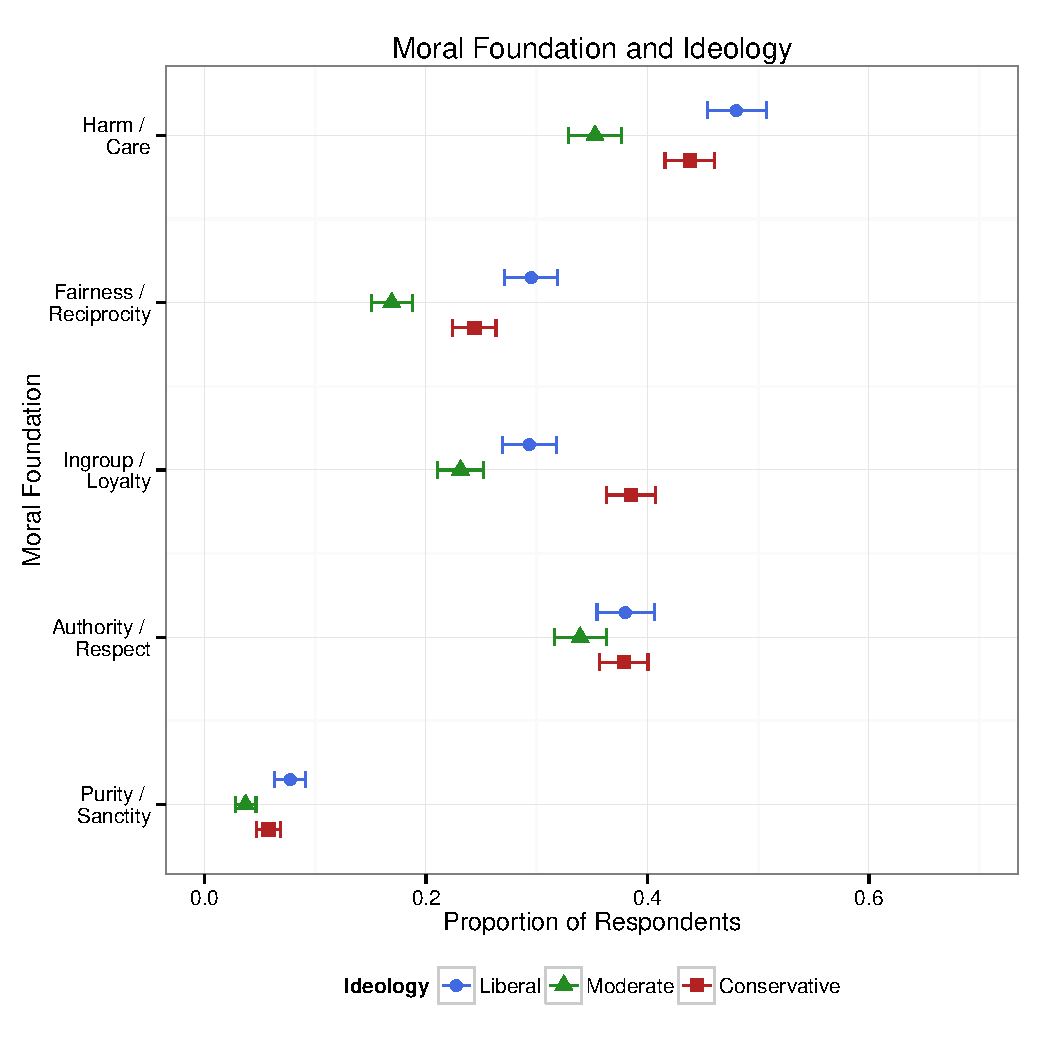
\includegraphics[scale=.5]{../calc/fig/p1_mft_ideol.pdf}
\caption{Moral foundations and ideology}\label{fig:mft_ideol}
\end{figure}

Looking first at the result for 2012 (lower part of Figure~\ref{fig:mft_ideol}), the patterns are largely consistent with our theoretical expectations. Liberals were more likely than conservatives or moderates to mention the harm/care foundation. Almost half of the respondentes identifying as liberals mentioned words belonging to the harm/care category in their responses. Furthermore, they were more likely than conservatives to mention the fairness/reciprocity foundation. This pattern is consistent with Moral Foundations Theory, as is the tendency for more conservatives to reference the ingroup/loyalty foundation than liberals or moderates. There were some notable contradictions, however. Liberals used fewer fairness/reciprocity words than authority/respect words. Indeed, the proportion of liberal respondents referencing authority/respect is almost identical to the proportion of conservatives mentioning authority/respect. This result is inconsistent with previous research by moral foundations scholars.

The fact that the purity/sanctity foundation was almost never mentioned by any of the respondents is surprising, since other studies found that the purity/sanctity foundation plays a very important role when looking at ideological differences \citep{koleva2012tracing}. This result suggests that subsequent analyses of survey responses might necessitate a revision of the moral foundation dictionary, since the terms contained in the dictionary might not be relevant enough for political evaluations. Accordingly, some of the words (e.g. in the case of purity/sanctity) are just too uncommon in the political context. Due to the very rare mentioning of the purity/sanctity dimension, the subsequent analyses will only concentrate on the remaining four moral foundations.

Turning to the results for 2008, there are fewer patterns that are consistent with Moral Foundations Theory. Indeed, the only difference between liberals and conservatives that is significant is the proportion of respondents referencing the ingroup/loyalty foundation. One potential explanation for the inconsistency across years is the fact that the open-ended responses were recorded in a more indirect manner in 2008. Many responses in 2008 consist of shorter summaries of the responses in verbatim. The sample size in 2008 is also much smaller, which explains the higher uncertainties around the estimated proportions.

Instead of looking at the aggregation of all survey items, we can also investigate the patterns in smaller subsets of responses (see Appendix~\ref{app:oview}). For example, taking into account only open-ended responses related to the evaluations of parties \textit{or} candidates shows the same basic patterns as in the pooled analysis. The results are also similar if respondents are differentiated by partisanship rather than political ideology. Overall, these results provide an inconclusive picture on the moral foundations of political reasoning. While some patterns are consistent with our theoretical expectations in 2012 (e.g. harm/care), they fail to be clearly replicated in 2008.

In a subsequent step, I estimated logit models using ideology (and several control variables) to predict the individual probability of referring to each of the moral foundations (excluding purity/sanctity) in both surveys. Note that all models control for the total number of words used by each respondent for their open-ended responses.\footnote{The full logistic regression results are presented in the appendix, Table~\ref{tab:m1_mft}}. Figure~\ref{fig:m1_mft} displays the expected change in predicted probabilities to mention each moral foundation when comparing liberals and conservatives while holding all other variables constant at their respective means, along with 95\% confidence intervals. Again, equivalent to the discussion of Figure~\ref{fig:mft_ideol}, the responses for each individual were collapsed such that the dependent variables indicate whether any of their responses contained a reference to the moral foundations as identified by the dictionary. 

\begin{figure}\centering
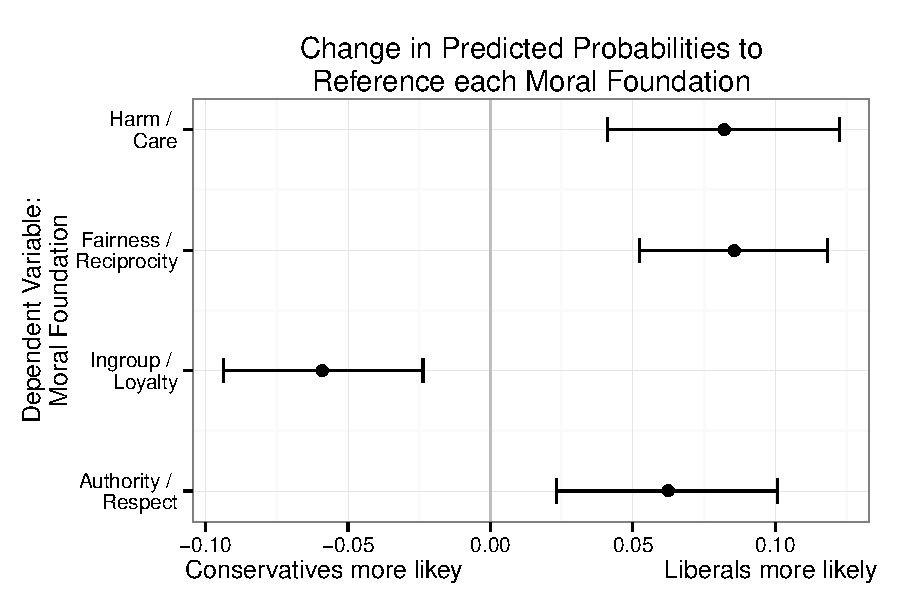
\includegraphics[scale=.5]{../calc/fig/m1_mft.pdf}
\caption{Difference in predicted probabilities to reference each moral foundation between liberals and conservatives}\label{fig:m1_mft}
\end{figure}

Positive values indicate a higher probability to mention the respective moral foundation in a response among respondents who identified as liberals, while negative values indicate a higher probability among conservatives. In 2012, the effects are consistent with the first hypothesis for three out of four moral foundations. Liberals are significantly more likely to mention harm/care and fairness/reciprocity when evaluating political parties and candidates than liberals. The probability of mentioning a word connected to the harm/care foundation is about 7.5 percentage points higher among liberals than conservatives. The effect is of similar size for the fairness/reciprocity dimension. Conversely, being conservative increases the likelihood of mentioning words that belong to the category of ingroup/loyalty by about 5 percentage points. However, liberals are significantly more likely to reference the moral foundation of authority/respect when evaluating political actors. This result is inconsistent with previous evidence regarding the endorsement of this foundation by conservatives. Furthermore, many of the effects from 2012 are not replicated when analyzing the 2008 ANES. Again, this may be due to the fact that the open-ended responses were recorded in a more indirect and summarized way than in 2012.

I conducted auxiliary analyses to probe the robustness of the patterns in Figure~\ref{fig:mft_ideol} and \ref{fig:m1_mft} and especially to investigate alternative explanations for the inconsistent finding regarding the moral foundation of authority/respect (detailed results are included in Appendix~\ref{app:robust}). On the one hand, they could indicate that the unidimensional conceptualization of ideology, which has been used in most studies analyzing moral foundations theory, is too simplistic in order to describe systematic individual differences. I repeated the analyses using a two-dimensional conceptualization of ideology differentiating between a social as well as an economic dimension as proposed by \citet{feldman2014understanding}. While providing a more detailed picture for the dimensions of harm/care (driven especially by the economic dimension) and fairness/reciprocity (driven especialy by the social dimension), the results for authority/respect are similar to the first analysis. 

The inconsistent results for the authority dimension might also be an artifact due to some peculiarity of the moral foundations dictionary. There might be signal words that are attributed to the authority/respect dimension and especially salient when talking about Barack Obama. For example, the moral foundations dictionary includes ``leader'' as a signal word for the authority/respet dimension. It could therefore be argued that the inconsistent finding is simply due to the fact that Obama is often considered as a ``good leader'' among his supporters. In order to examine this issue, I repeated the analyses after omitting ``leader'' from the moral foundations dictionary. The results do not change substantially.

More detailed analyses of the open-ended responses suggest that liberals were more likely to reference the authority dimension as a virtue (after disaggregating the moral dictionary by valence, see \url{www.moralfoundations.org}), when talking about positive aspects about parties and candidates, as well as when discussing their in-party candidate. It appears that the Democratic candidate in both elections (Barack Obama) was partly viewed favorably by supporters due to considerations related to the moral foundation of authority/respect. This result can be seen as a first indication that the differences in moral reasoning between liberals and conservatives are contingent upon the respective political environment.

The results discussed so far indicate that there are indeed important differences between liberals and conservatives in terms of their reliance on different moral considerations when evaluating political parties and candidates. However, the patterns cannot be described as unequivocally consistent with the predictions of Moral Foundations Theory. The fact that some foundations showed contrary patterns, as well as the failure to replicate the findings across years suggests that the reliance on moral foundations might be more context-specific than previously theorized.


\subsubsection{Determinants of Moral Reasoning}

Having shown that liberals and conservatives indeed differ with regard to the moral foundations they emphasize when evaluating political actors, I investigate whether the reliance on moral considerations is a product of exposure to political discourse. I predict the probability of mentioning any moral foundation with a series of logit models in which political sophistication, political media exposure, and frequency of political discussions are the key independent variables. Figure~\ref{fig:m3_learn} depicts the respective predicted probabilities when each independent variable (knowledge, media exposure, discussion) is increased from its empirical minimum value to its empirical maximum value, holding all other variables (including the number of words in each individual response) constant at their means.\footnote{Full model results are displayed in the appendix, Table~\ref{tab:m3_learn}.}

\begin{figure}\centering
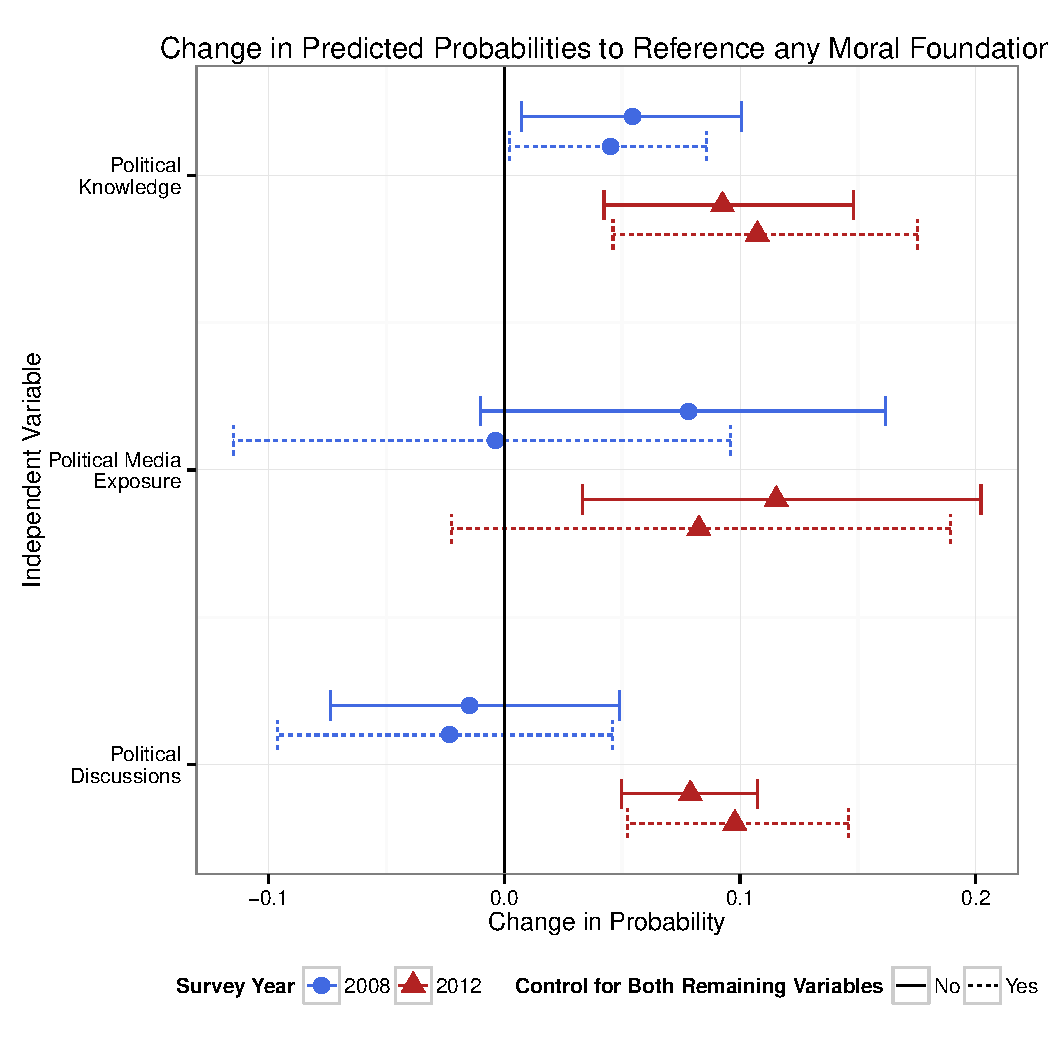
\includegraphics[scale=.5]{../calc/fig/m3_learn.pdf}
\caption{Change in predicted probabilities to reference any of the moral foundations depending on political knowledge, media exposure, and frequency of political discussions}\label{fig:m3_learn}
\end{figure}

The results show, that most variables (except political discussions in 2008) have a positive effect on the individual probability to make use of moral foundations when evaluating political parties and candidates. Higher political sophistication, higher exposure to political media and news, as well as more frequent political discussions increase the probability that individuals rely on moral considerations. Thereby, citizens \textit{learn} to embed moral reasoning in their political evaluations. While moral intuitions themselves might well be innate, the extent to which individuals make use of these intuitions when thinking about politics and evaluating political actors may be more context-dependent and subject to individual heterogeneity.

The significant positive effect of frequent political discussions in 2012 (even after controlling for the two remaining variables, political knowledge and media exposure), is especially interesting in this context. Citizens, who engage in frequent political arguments are more likely to use moral considerations when evaluating candidates and parties. This result could suggest that morality in politics plays an important role as a rhetorical tool utilized to convince others of certain political views. Overall, positive relationships between political knowledge, media exposure, and political discussions and moral reasoning are quite robust, even while controlling for individual response lengths. It is worth noting again that all analyses reported here include the length of individual responses as control variables, which should at least partly account for potential confounding factors such as general effects of increased political literacy on the complexity of open-ended responses.

\begin{figure}\centering
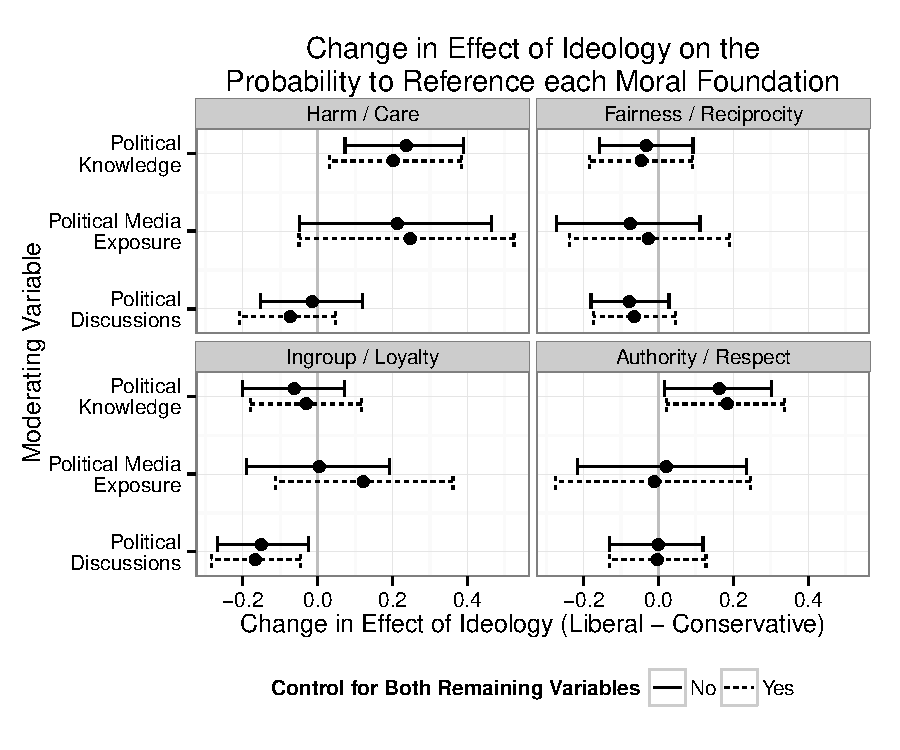
\includegraphics[scale=.5]{../calc/fig/m3b_learn.pdf}
\caption{Change in effect of ideology on predicted probabilities to reference each of the moral foundations moderated by political knowledge, media exposure, and frequency of political discussions (difference-in-difference)}\label{fig:m3b_learn}
\end{figure}

In addition to examining the reference to moral foundations \textit{in general}, we can also consider whether the effects of political discourse increase the differences in the emphasis on specific dimensions between liberals and conservatives. Figure~\ref{fig:m3b_learn} presents the change in the effect of ideology on the probability to reference each of the moral foundations moderated by political knowledge, media exposure, and frequency of political discussions. Thus, each point in the figure displays the interaction effect between knowledge, media exposure, and discussion, as well as ideology as a difference-in-difference in predicted probabilities while holding all other variables constant at their respective means. For example, the positive effect for political knowledge on the probability to reference the harm/care foundation in 2012 (top left part in the figure) indicates, that when political knowledge is increased from its empirical minimum to its maximum, the difference between liberals and conservatives is increased such that liberals are about 25 percentage points more likely to mention words belonging to the harm/care foundation than conservatives. In other words, positive effects imply that the gap between liberals and conservatives on the respective dimension is increased in favor of liberal respondents. Negative effects, on the other hand, indicate that the gap between liberals and conservatives is increased with conservatives becoming more likely to reference the respective moral dimension.

In order to interpret these difference-in-difference effects, consider again the basic findings reported in Figure~\ref{fig:m1_mft}. The estimates showed that on average, liberals were more likely to refernce the foundations of harm/care, fairness/reciprocity, and authority/respect, whereas conservatives were more likely to mention considerations related to the ingroup/loyalty dimension. Focusing on the effects in 2012 in Figure~\ref{fig:m3b_learn}, we see that for individuals with high political knowledge and media exposure, the difference between liberals and conservatives in terms of the harm/care foundation was more pronounced: the difference between liberals and conservatives is increased such that liberals are even more likely to reference this dimension compared to conservatives. While we do not observe any meaningful moderation effects for the fairness/reciprocity dimension, there is some evidence that the ideological gap in the ingroup/loyalty dimension is higher for respondents who discuss politics more frequently, as well as in the authority/respect dimension for respondents with high political knowledge. Again, these results are only apparent in 2012 and cannot be replicated in 2008.

Overall, political knowledge, media exposure, and political discussions do not only affect general levels of moral reasoning but also moderate the ideological gap between liberals and conservatives. This finding indicates that the effects of political discourse cannot be reduced to an artifact of differences in political literacy and more elaborate argumentation. Some portion of the ideological differences in emphasis on moral foundations can therfore be described as a product of learning in the political environment.


\subsubsection{Investigating the Political Relevance of Moral Reasoning}

Previous research relying on the MFQ linked moral foundations to a wide array of political outcomes, such as turnout \citep{johnson2014ideology}, candidate preferences \citep{iyer2010beyond}, and voting behavior \citep{franks2015using}. In the present study, it is argued that measures like the MFQ capture a latent predisposition for certain moral dimensions rather than directly assessing the actual reliance on moral considerations in political reasoning. In order to emphasize the importance of the distinction between moral foundations and explicit moral reasoning, it has to be examined whether the latter is indeed politically relevant. Thus, after showing similar ideological patterns in references to moral foundations based on open-ended survey responses and analyzing the extent to which moral reasoning (and the ideological gap therein) are contingent upon exposure to political discourse, we will now investigate whether the measure of moral reasoning employed here affects relevant political outcomes.

As a first step, we will examine whether references to moral foundations affect political participation. Figure~\ref{fig:m2b_vote} displays the results of logit models predicting individual turnout as a function of individual references to moral foundations (as well as the regular set of control variables used in the previous analyses).

\begin{figure}[ht]\centering
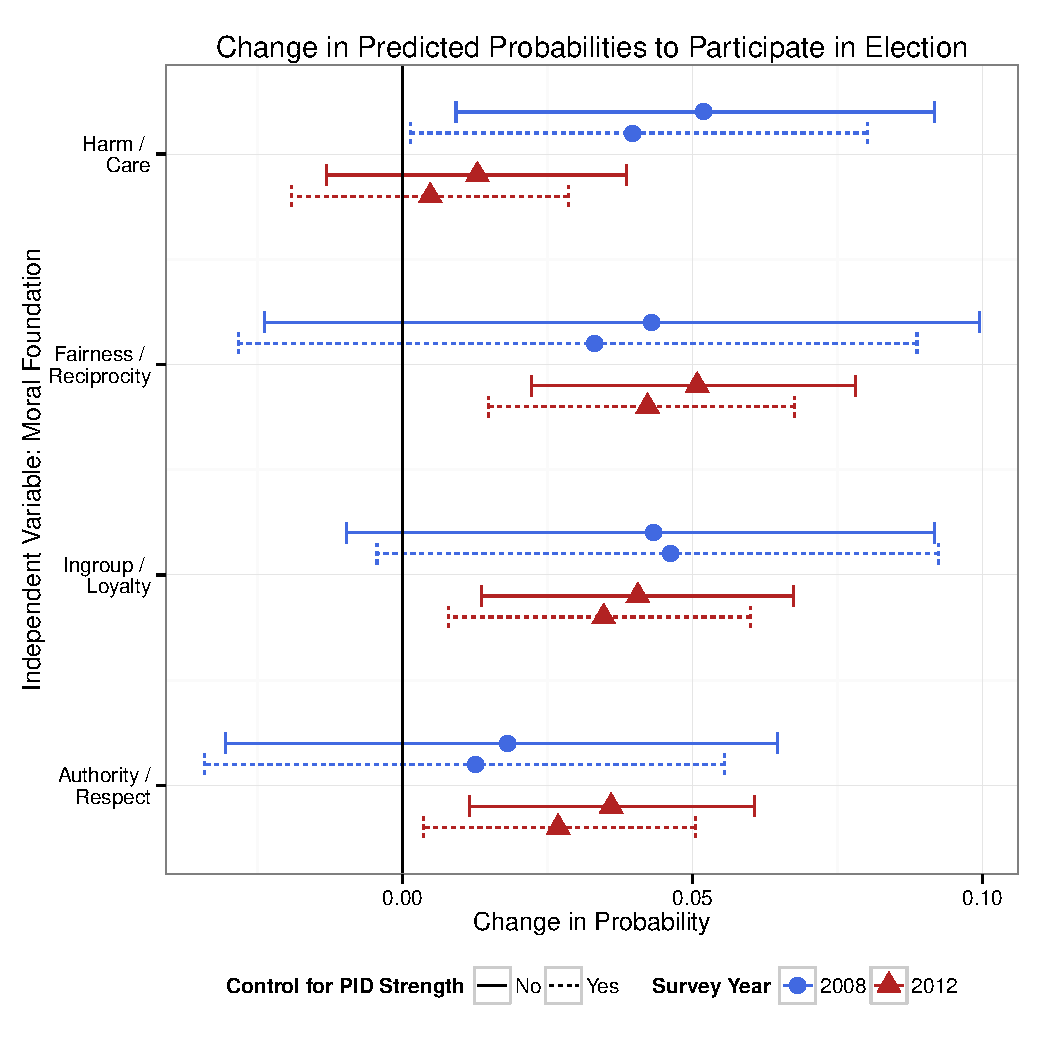
\includegraphics[scale=.5]{../calc/fig/m2b_vote.pdf}
\caption{Change in predicted probabilities to participate in election depending on references to specific moral foundations}\label{fig:m2b_vote}
\end{figure}

Each of the moral foundations have a positive effect on the predicted probabilities of participating in the election. For example, if a respondent mentions considerations related to fairness/reciprocity when discussing his or her political preferences, the probability of turning out to vote is increased by amost 5 percentage points, holding all other variables constant at their respective means. While not all the effects are statistically significant, the overall pattern is clear. References to any moral foundation increase the probability of voting. Note that the estimates are based on models that already take into account the length of individual responses. Furthermore, most of the effects stay significant and are only reduced marginally after controlling for the strength of individual party identification.

\begin{figure}[ht]\centering
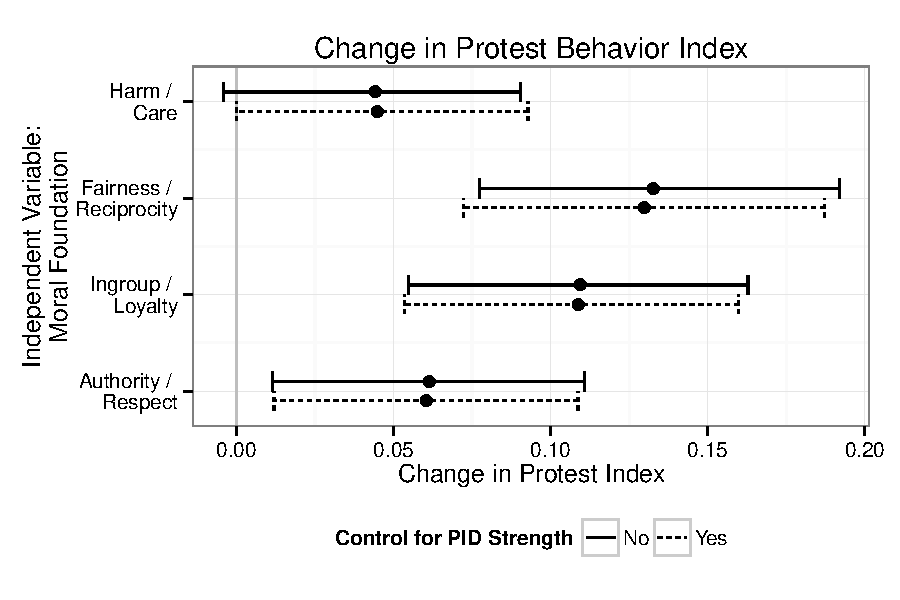
\includegraphics[scale=.5]{../calc/fig/m2e_part.pdf}
\caption{Change in protest behavior index depending on references to specific moral foundations}\label{fig:m2b_vote}
\end{figure}

The influence of moral reasoning extends to other forms of participation. Figure~\ref{fig:m2b_vote} displays estimates from a linear regression predicting protest behavior (participation in demonstration, displaying signs or campaign stickers, signing petitions) based on moral foundations. Again, references to moral foundations generally has positive effects on political engagement outside of the ballot box. Consider the effect of ingroup/loyalty in 2012 as an example. If respondents mentioned considerations related to this moral foundation, their additive protest index (ranging from 0 to 3) is increased by 0.1 points. This effect might not seem large, but bear in mind that the independent variable consists of a dichotomous indicator for references to any moral foundation in a set of open-ended questions. The fact that we can recover consistent and statistically significant effects on political participation in such a context (even after controlling for strength of party identification and the length of individual responses) is therefore quite meaningful.

Overall then, the analyses indicate that moral reasoning is positively associated with political engagement. That said, the analyses presented here are not sufficient to make a strong causal claim about the direction of this relationship. Yet, the results suggest that moral reasoning (as measured by open-ended survey responses) is powerfully related to different forms of political participation and engagement.

\begin{figure}[ht]\centering
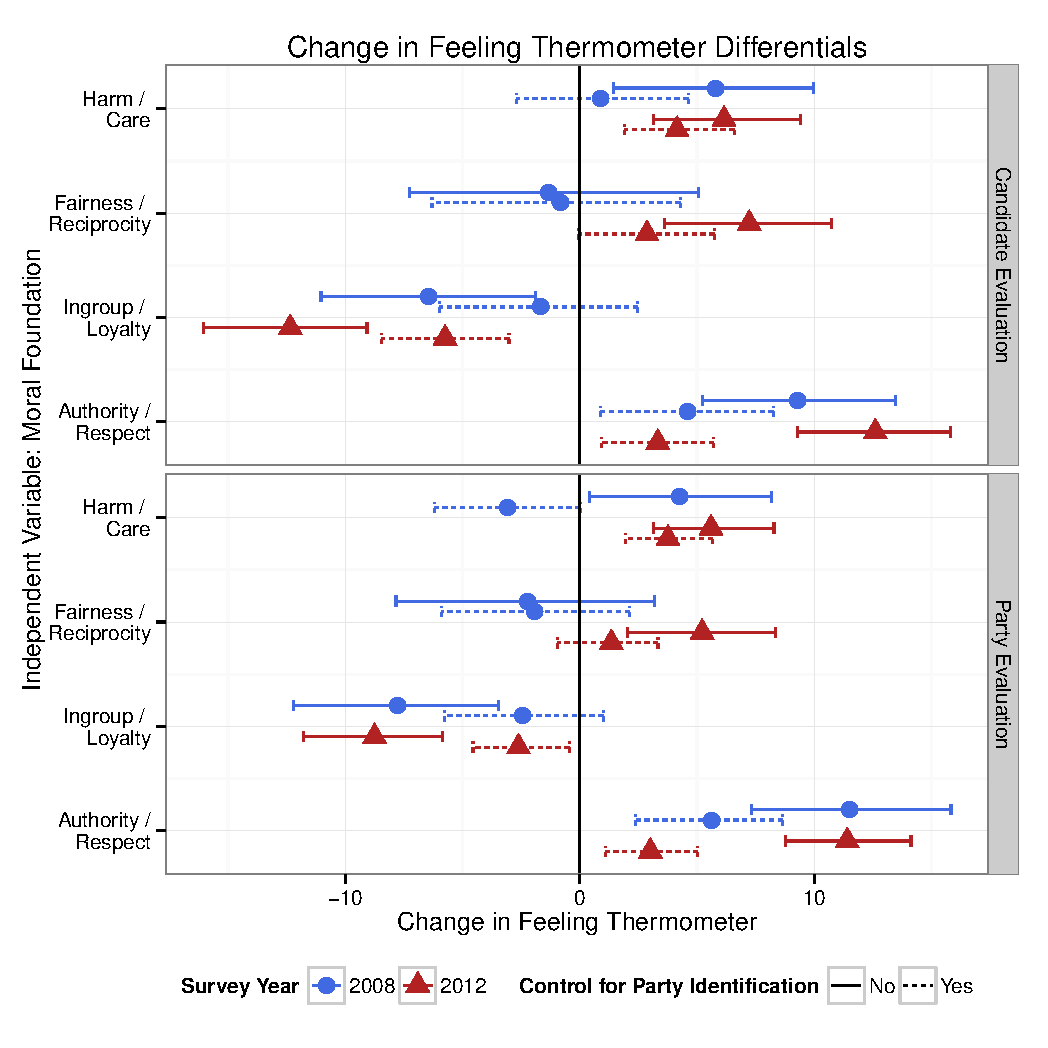
\includegraphics[scale=.5]{../calc/fig/m2f_vote.pdf}
\caption{Effect of moral foundations on feeling thermometer differentials (candidates and parties)}\label{fig:m2f_vote}
\end{figure}

In the next step, we turn to the relationship of moral reasoning and political preferences themselves. Figure~\ref{fig:m2f_vote} presents the results of linear regressions of moral foundations predicting the change in the feeling thermometer differential between the Republican and the Democratic Presidential candidate (top part of the figure) and the change in the feeling thermometer differential between the Republican and Democratic party. Positive values indicate more favorable evaluations for the Democratic candidate or party and negative values indicate more favorable evaluations of the Republican candidate or party. The patterns are largely consistent with the previous results on ideological differences. Individuals who mention considerations related to harm/care, fairness/reciprocity, and authority/respect evaluate the Democrative candidates on average 5 points higher than the Republican candidates (on a 100 point scale). On the other hand, if individuals emphasized the ingroup/loyalty dimension, they reported stronger preferences for the Republican candidates. These effects are robust after controlling for individual party identification. Thus, in both analyses in Figure~\ref{fig:m2f_vote}, we observed sizeable and significant effects for the influence of moral reasoning. This result is especially noteworthy given that respondents were not explicitly asked about morality. Furthermore, we do not distinguish between statements for either party or between positive and negative statements when constructing the indicators denoting moral references. Even though we are simply looking at the content of the collection of all positive and negative statements about both candidates and parties, we observe consistent and substantial effects on subsequent evaluations.

Lastly, Figure~\ref{fig:m2_vote} finally presents the changes in expected probabilities of voting for the Democratic (vs. the Republican) presidential candidate in the 2008 and 2012 election for individuals mentioning the moral foundations in their open-ended responses. The estimated probabilities are based on logit models including dummies for each moral foundation as independent variables as well as several sociodemographic control variables, which were held constant at their mean values when calculating expected values.\footnote{Full model results are displayed in the appendix, Table~\ref{tab:m2_vote}.}

\begin{figure}[ht]\centering
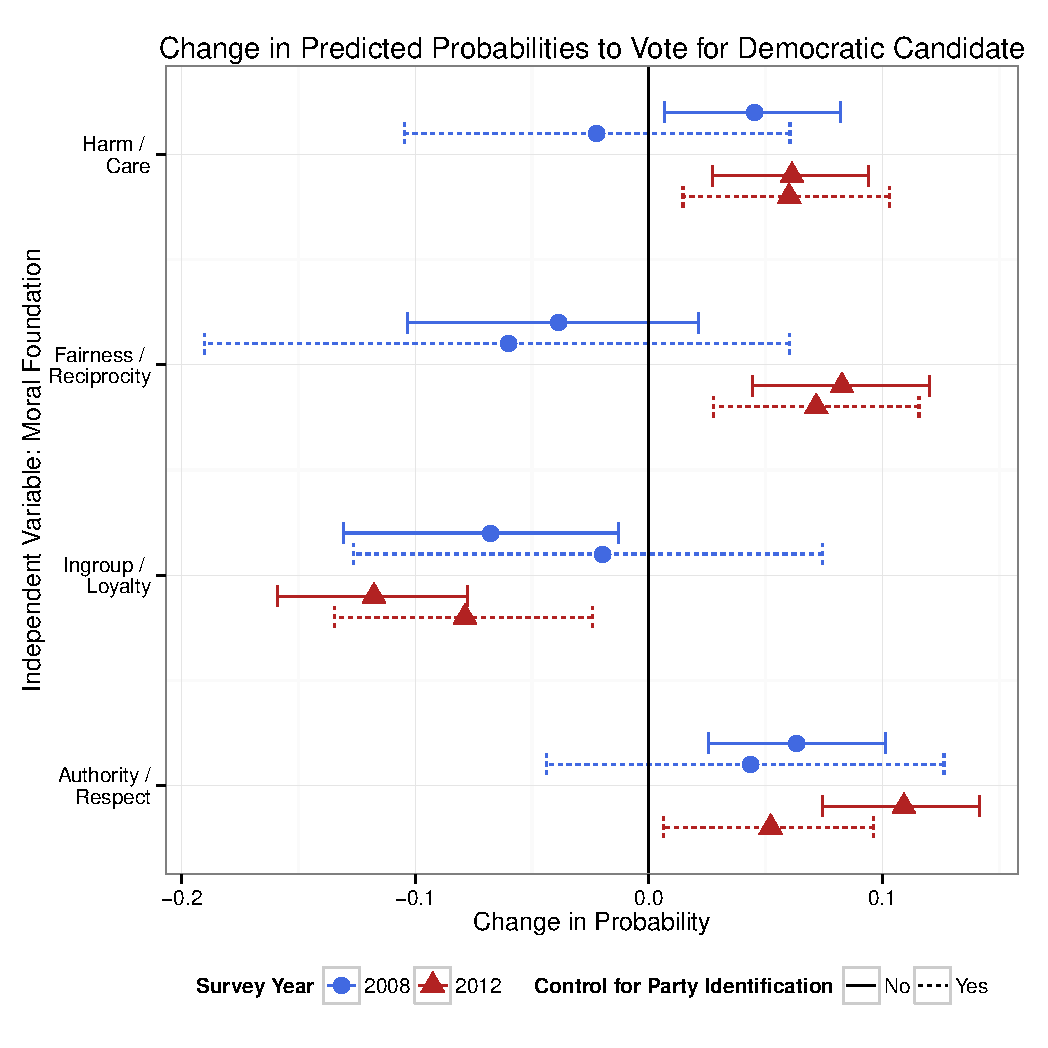
\includegraphics[scale=.5]{../calc/fig/m2_vote.pdf}
\caption{Change in predicted probabilities to vote for democratic candidate depending on references to specific moral foundations}\label{fig:m2_vote}
\end{figure}

While not all effects displayed in Figure~\ref{fig:m2_vote} are statistically significant (especially in 2008), the patterns are similar to the results presented thus far. Individuals who mentioned moral considerations related to the harm/care foundation are (slightly) more likely to vote for the Democratic candidate. In 2012, the effect for the fairness/reciprocity foundation is also positive: respondents who mentioned this foundation were more likely to vote for Barack Obama than for Mitt Romney. In 2008, by contrast, the effects are negative and insignificant. Respondents who emphasized the ingroup/loyalty foundation, on the other hand, were less likely to vote for the Democratic candidate in both elections. While these results appear to be relatively consistent with Moral Foundations Theory, we see again that the effect for the authority/respect foundation deviates from our expectations: respondents mentioning this foundation were more likely to vote for the presidential candidate. Overall, Figure~\ref{fig:m2_vote} shows that it is possible to predict voting behavior simply by observing the moral dimensions of the respondents' political reasoning, without taking into account which candidate they described, and whether the description is framed positively or negatively. Moreover, most of these effects are even persistent when controlling for individual party identification.


\section{Conclusion}

The goal of this paper was to investigate whether the ideological differences in the emphasis on moral foundations manifests itself in individual reasoning about political actors. It was argued that the analyses of open-ended survey responses can provide important insights beyond previous research because it allows to evaluate whether citizens make references to moral considerations in a political context that does not induce an explicit connection to morality. Furthermore, it was argued that the reliance on moral reasoning as such is moderated by political knowledge, media exposure, and political discussions. The emphasis of specific moral foundations, in turn, was expected to influence important political outcomes such as participation, candidate evaluations, and voting behavior.

The empirical evidence discussed in this paper is only partly consistent with previous results on moral foundations and ideology. The first hypothesis, which predicted systematic patterns in the emphasis on moral considerations among liberals and conservatives, was supported for three out of four foundations in 2012. Liberals are more likely to mention considerations related to harm/care and fairness/reciprocity when discussing their political preferences, whereas conservatives are more likely to emphasize the moral foundation of ingroup/loyalty.

According to the second hypothesis, it was expected that individuals show heterogeneity in terms of their tendency to rely on moral reasoning. The results indicated that political knowledge, discussions, as well as media consumption increase the reliance on moral considerations. Thus, the evidence suggests that moral reasoning is part of a broader political learning process. At least in some cases, this learning process appears to imply an increased differentiation between liberals and conservatives in terms of the focus on specific foundations as described by Moral Foundations Theory.

The last part of the analyses focused on the political relevance of moral reasoning as conceptualized based on open-ended survey responses. The results here revealed consistent relationships between individual moral foundations and different forms of political participation, candidate evaluation, and voting behavior. As such, moral reasoning measured using open-ended survey responses is a politically meaningful and influential concept.

The contributions of this paper are therefore twofold. It adds to the existing literature on moral foundations by providing new insights into the mechanisms underlying its relationship with ideology. Furthermore, from a general methodological perspective, the paper emphasizes the potential benefits of incoporating open-ended survey responses in research focusing on the determinants and structure of ideology and political reasoning. In the context of moral foundations, the paper shows that we can directly assess moral reasoning in surveys that do not contain the MFQ or related measures, simply by relying on open-ended survey responses.

However, there are some issues that should be raised regarding the analyses presented here. The fact that purity/sanctity was almost never mentioned as well as the inconsistent effect of ideology on the authority/respect dimension could be attributed to the fact that the moral foundations dictionary was originally used for the analyses of sermons. Accordingly, subsequent analyses could revise the dictionary in order to make it more applicable for the analyses of survey responses. Furthermore, it should be noted that the modelling strategy based on multiple logistic regressions assumes independence between the different response categories. This assumption does not seem to be plausible since the reference to a specific moral foundation might well affect how often individuals mention other considerations. While a multinomial logit / conditional logit framework is also not feasible due to the fact that individuals can fall in several categories, other model approaches for non-exclusive multinomial choices might improve the empirical analyses \citep[see for example][]{gilbert2007models}.

An alternative approach to the analysis of open-ended survey responses could be the implementation of structural topic models as described by \citet{roberts2014structural}: instead of using explicit word lists to identify moral reasoning, it would possible to identify specific topics in open-ended responses that are consistent with the moral foundations described by \citet{haidt2008moral} \citep[see also][]{lin2008joint}.

Another issue that remains unresolved is the question of causality. \citet{graham2009liberals} rightfully stated that the causal nature of the relationship between moral foundations and ideology is not yet established. More specifically, their study did not settle whether individuals first identify as liberal or conservative and then adapt their respective moral judgments, or whether moral considerations shape and structure subsequent ideological thinking itself. Recent research focusing on elite influences on moral reasoning suggests that political elite rhetoric plays an important role in shaping individual moral judgment. These results indicate that the influence of moral judgments in politics is indeed context-specific \citep[see for example][]{clifford2013words,clifford2015concerns}. The evidence presented here would suggest a similar causal mechanism. However, resolving this issue requires additional research where moral reasoning is manipulated experimentally.

It would also be worth investigating whether the patterns regarding moral reasoning change over larger periods of time using this method in order to further establish the context-specific nature of moral reasoning. At this time, however, full-text open-ended survey responses are not available in the ANES prior to 2008.

Irrespective of these reservations, the analyses of open-ended survey responses can provide important and valuable insights in the context of moral foundations and the individual underpinnings of political ideology. Utilizing available responses to open-ended survey questions provides a useful and still largely neglected data source to investigate these and other important research questions from novel perspectives.


\clearpage
\bibliographystyle{/data/Copy/1-src/lit/apsr2006}
\bibliography{/data/Copy/1-src/lit/Literature}

\clearpage\flushleft\footnotesize\singlespacing
\appendices
\appendixpage
\startcontents[sections]
\printcontents[sections]{l}{1}{\setcounter{tocdepth}{2}}
\clearpage


\section{Moral Foundations Dictionary}
\renewcommand\thefigure{\thesection.\arabic{figure}}
\renewcommand\thetable{\thesection.\arabic{table}}
\setcounter{figure}{0}
\setcounter{table}{0}

\textit{Sources:}\\
\citet{graham2009liberals}, as well as \url{http://www.moralfoundations.org/}
\vspace{.5cm}

\textit{Note:}\\
Words with (*) indicate that the word stem rather than the exact word was matched in the open-ended survey responses.
\vspace{.5cm}

\textbf{Harm:}\\
safe*, peace*, compassion*, empath*, sympath*, care, caring, protect*, shield, shelter, amity, secur*, benefit*, defen*, guard*, preserve, harm*, suffer*, war, wars, warl*, warring, fight*, violen*, hurt*, kill, kills, killer*, killed, killing, endanger*, cruel*, brutal*, abuse*, damag*, ruin*, ravage, detriment*, crush*, attack*, annihilate*, destroy, stomp, abandon*, spurn, impair, exploit, exploits, exploited, exploiting, wound*
\vspace{.5cm}

\textbf{Fairness:}\\
fair, fairly, fairness, fair*, fairmind*, fairplay, equal*, justice, justness, justifi*, reciproc*, impartial*, egalitar*, rights, equity, evenness, equivalent, unbias*, tolerant, equable, balance*, homologous, unprejudice*, reasonable, constant, honest*, unfair*, unequal*, bias*, unjust*, injust*, bigot*, discriminat*, disproportion*, inequitable, prejud*, dishonest, unscrupulous, dissociate, preference, favoritism, segregat*, exclusion, exclud*
\vspace{.5cm}

\textbf{Ingroup:}\\
together, nation*, homeland*, family, families, familial, group, loyal*, patriot*, communal, commune*, communit*, communis*, comrad*, cadre, collectiv*, joint, unison, unite*, fellow*, guild, solidarity, devot*, member, cliqu*, cohort, ally, insider, foreign*, enem*, betray*, treason*, traitor*, treacher*, disloyal*, individual*, apostasy, apostate, deserted, deserter*, deserting, deceiv*, jilt*, imposter, miscreant, spy, sequester, renegade, terroris*, immigra*
\vspace{.5cm}

\textbf{Authority:}\\
obey*, obedien*, duty, law, lawful*, legal*, duti*, honor*, respect, respectful*, respected, respects, order*, father*, mother, motherl*, mothering, mothers, tradition*, hierarch*, authorit*, permit, permission, status*, rank*, leader*, class, bourgeoisie, caste*, position, complian*, command, supremacy, control, submi*, allegian*, serve, abide, defere*, defer, revere*, venerat*, comply, defian*, rebel*, dissent*, subver*, disrespect*, disobe*, sediti*, agitat*, insubordinat*, illegal*, lawless*, insurgent, mutinous, defy*, dissident, unfaithful, alienate, defector, heretic*, nonconformist, oppose, protest, refuse, denounce, remonstrate, riot*, obstruct
\vspace{.5cm}

\textbf{Purity:}\\
piety, pious, purity, pure*, clean*, steril*, sacred*, chast*, holy, holiness, saint*, wholesome*, celiba*, abstention, virgin, virgins, virginity, virginal, austerity, integrity, modesty, abstinen*, abstemiousness, upright, limpid, unadulterated, maiden, virtuous, refined, intemperate, decen*, immaculate, innocent, pristine, humble, disgust*, deprav*, disease*, unclean*, contagio*, indecen*, sin, sinful*, sinner*, sins, sinned, sinning, slut*, whore, dirt*, impiety, impious, profan*, gross, repuls*, sick*, promiscu*, lewd*, adulter*, debauche*, defile*, tramp, prostitut*, unchaste, wanton, profligate, filth*, trashy, obscen*, lax, taint*, stain*, tarnish*, debase*, desecrat*, wicked*, blemish, exploitat*, pervert, wretched*
\vspace{.5cm}

%\textbf{General:}\\
%righteous*, moral*, ethic*, value*, upstanding, good, goodness, principle*, blameless, exemplary, lesson, canon, doctrine, noble, worth*, ideal*, praiseworthy, commendable, character, proper, laudable, correct, wrong*, evil, immoral*, bad, offend*, offensive*, transgress*, honest*, lawful*, legal*, piety, pious, wholesome*, integrity, upright, decen*, indecen*, wicked*, wretched*


\clearpage
\section{Additional Tables and Figures - Overview}\label{app:oview}
\renewcommand\thefigure{\thesection.\arabic{figure}}
\renewcommand\thetable{\thesection.\arabic{table}}
\setcounter{figure}{0}
\setcounter{table}{0}

%%%%%%%%%%%%%%%%%%%%%%%%%%%%%%%%%%%%%%%%%%%%%%%%%%%%%%%%%%%%%%%%%%%%%%%
% APPENDIX DOES NOT INCLUDE ALL MODELS DISCUSSED IN THE MAIN PART YET %
%%%%%%%%%%%%%%%%%%%%%%%%%%%%%%%%%%%%%%%%%%%%%%%%%%%%%%%%%%%%%%%%%%%%%%%
% which tables and figures should be included

% latex table generated in R 3.2.2 by xtable 1.7-4 package
% Wed Sep 16 10:56:58 2015
\begin{table}[ht]
\centering
\begin{tabular}{lcc}
  \hline
 & N & Percent \\ 
  \hline
Spanish Interview (2008) & 94 & 4.05 \\ 
  Spanish Interview (2012) & 228 & 3.86 \\ 
  No Responses (Overall, 2008) & 158 & 7.09 \\ 
  No Responses (Overall, 2012) & 392 & 6.89 \\ 
  No Responses (Candidate Evaluations, 2008) & 328 & 14.13 \\ 
  No Responses (Candidate Evaluations, 2012) & 761 & 12.87 \\ 
  No Responses (Party Evaluations, 2008) & 584 & 25.15 \\ 
  No Responses (Party Evaluations, 2012) & 1503 & 25.41 \\ 
   \hline
\end{tabular}
\caption{Overview - Missing Open-Ended Responses} 
\label{tab:a1_mis}
\end{table}


\begin{figure}[ht]\centering
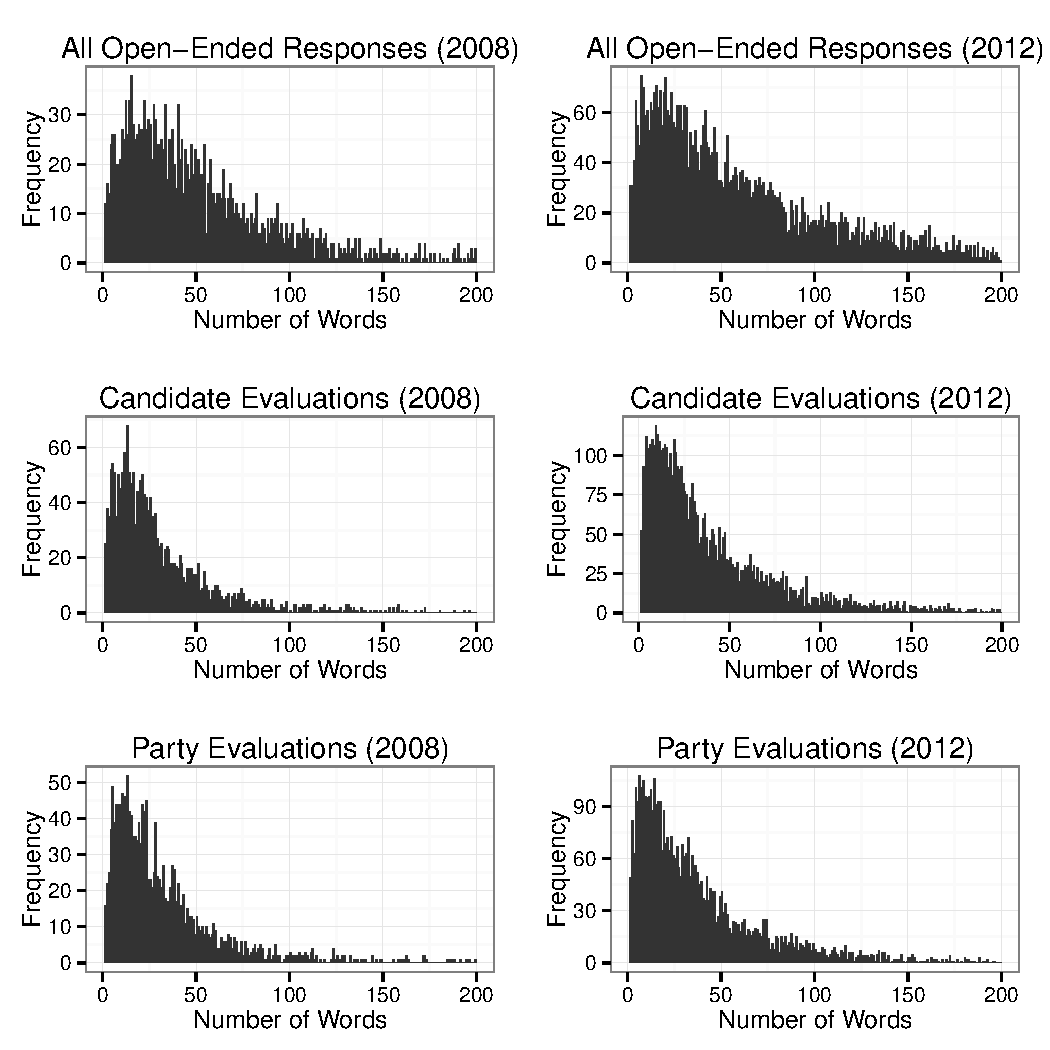
\includegraphics[scale=.6]{../calc/fig/a0_num.pdf}
\caption{Distribution of numbers of words in open-ended responses}\label{fig:a0_num}
\end{figure}

\begin{figure}\centering
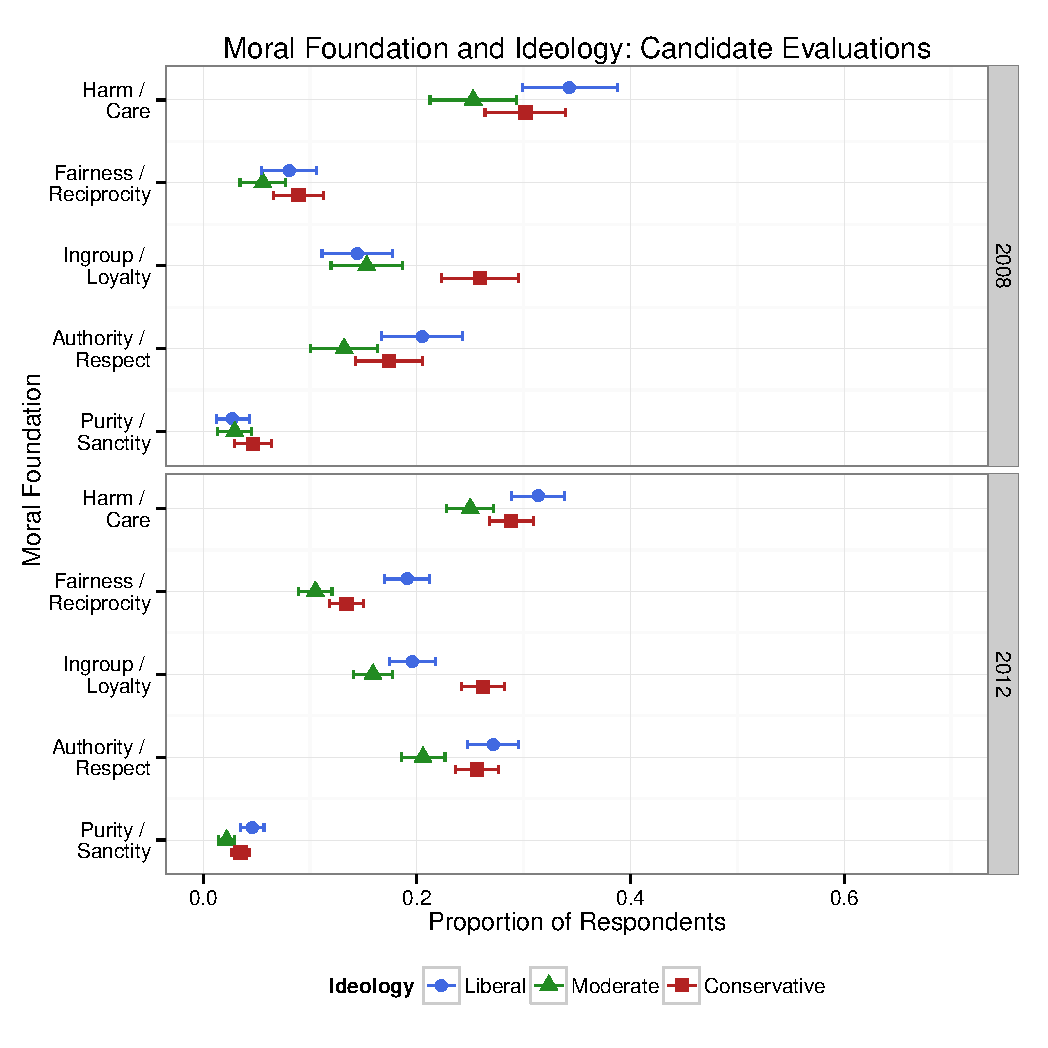
\includegraphics[scale=.4]{../calc/fig/p2_mft_ideol_ca.pdf}
\caption{Moral foundations and ideology (party evaluations)}\label{fig:mft_ideol_pa}
\end{figure}

\begin{figure}\centering
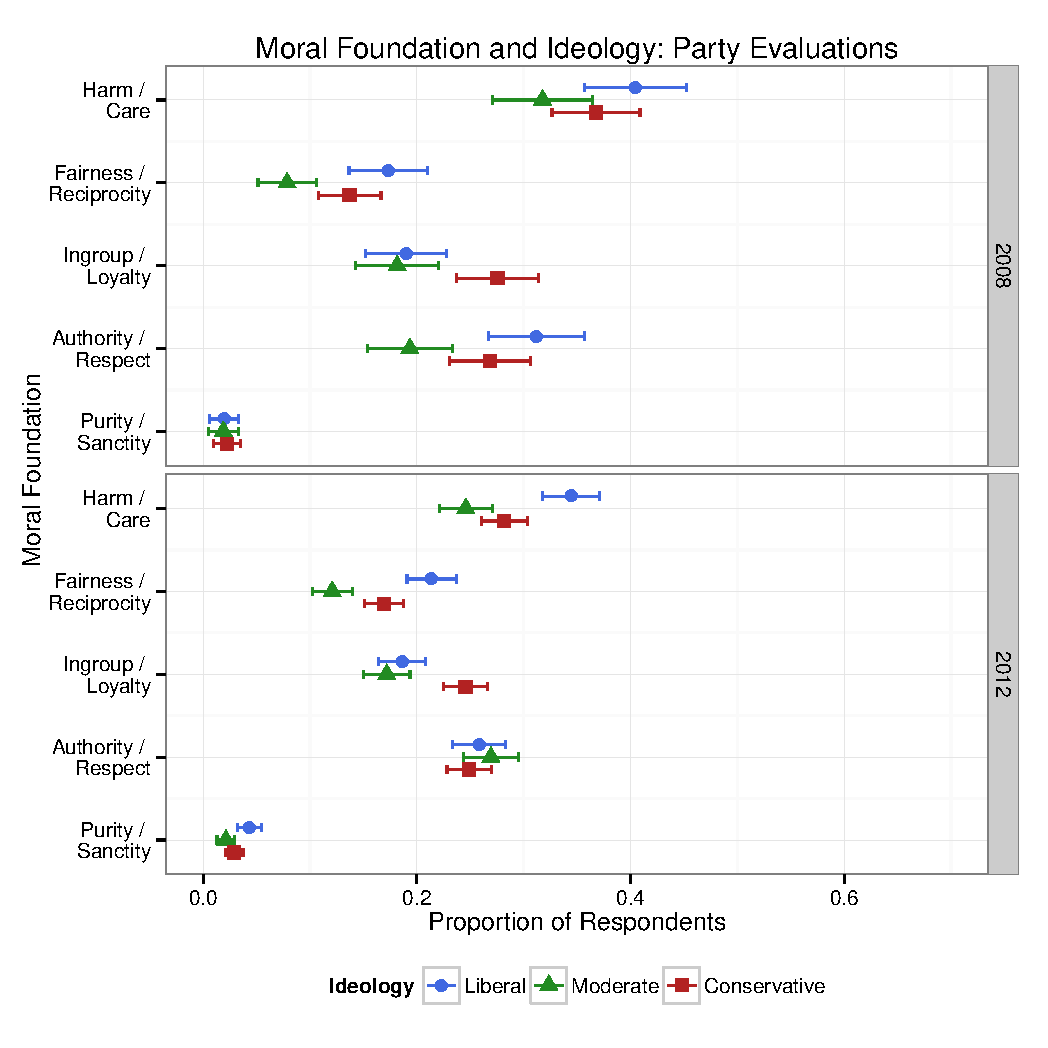
\includegraphics[scale=.4]{../calc/fig/p3_mft_ideol_pa.pdf}
\caption{Moral foundations and ideology (candidate evaluations)}\label{fig:mft_ideol_ca}
\end{figure}

\begin{figure}[ht]\centering
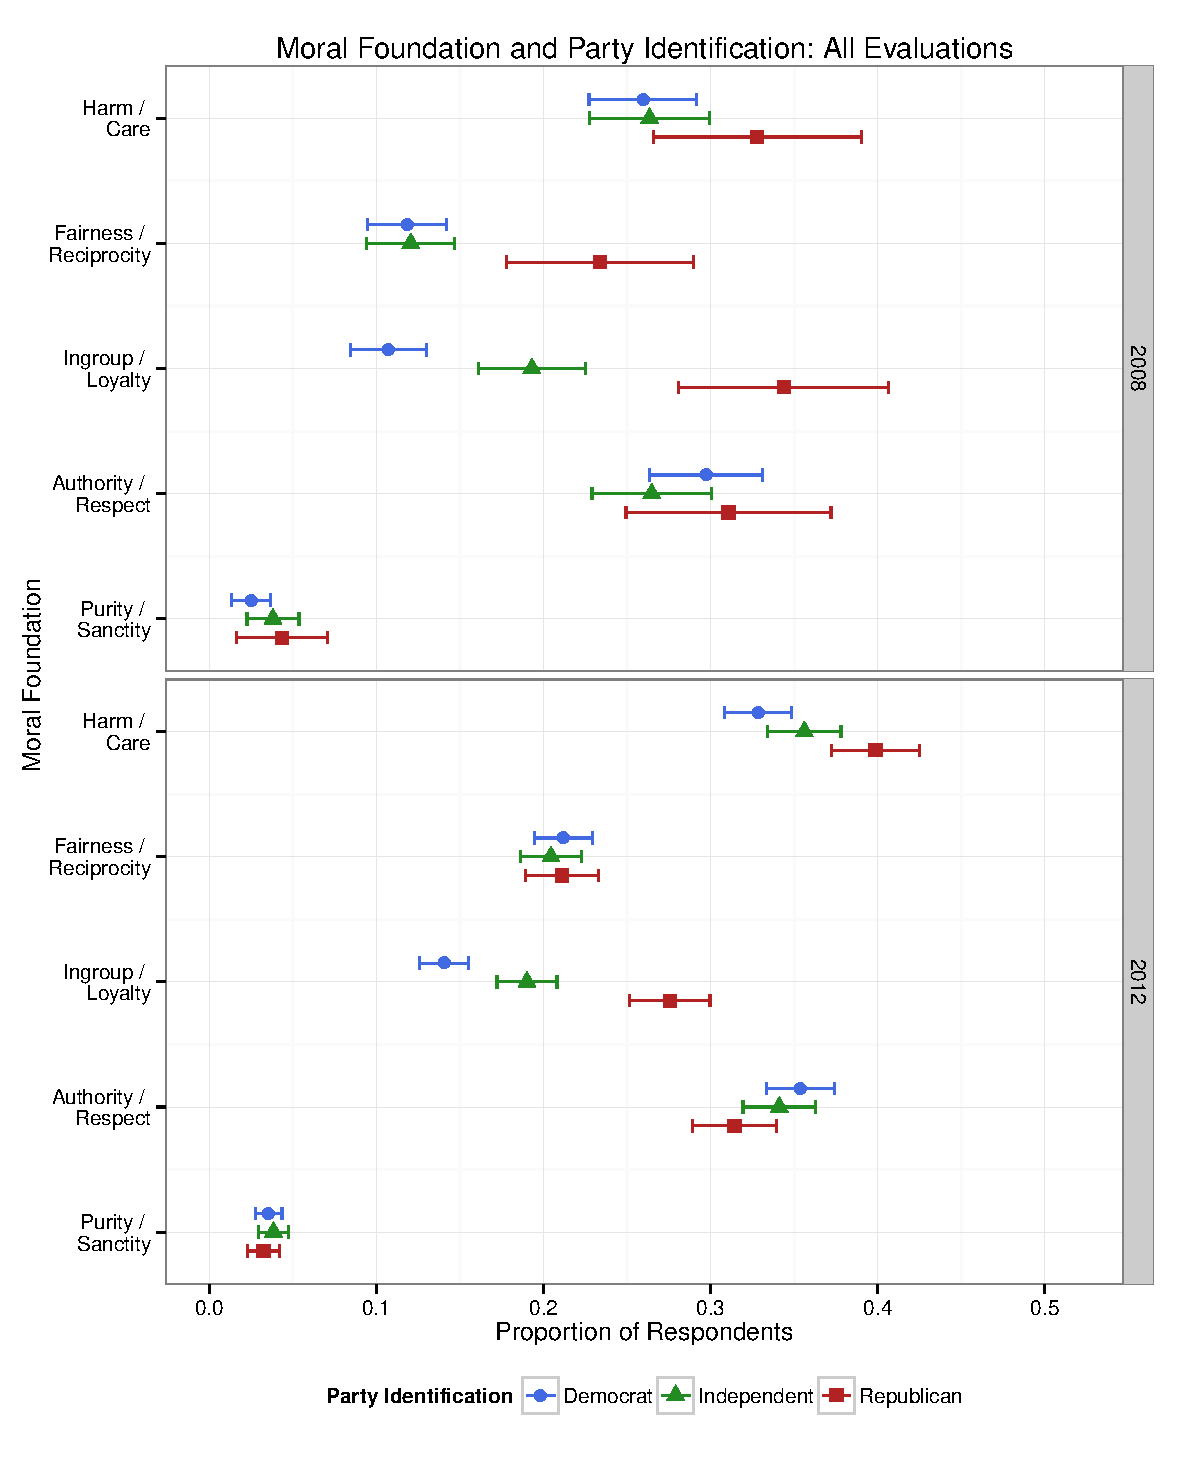
\includegraphics[scale=.4]{../calc/fig/a1_mft_pid.pdf}
\caption{Moral foundations and partisanship (all statements)}\label{fig:a1_mft_pid}
\end{figure}

\begin{figure}[ht]\centering
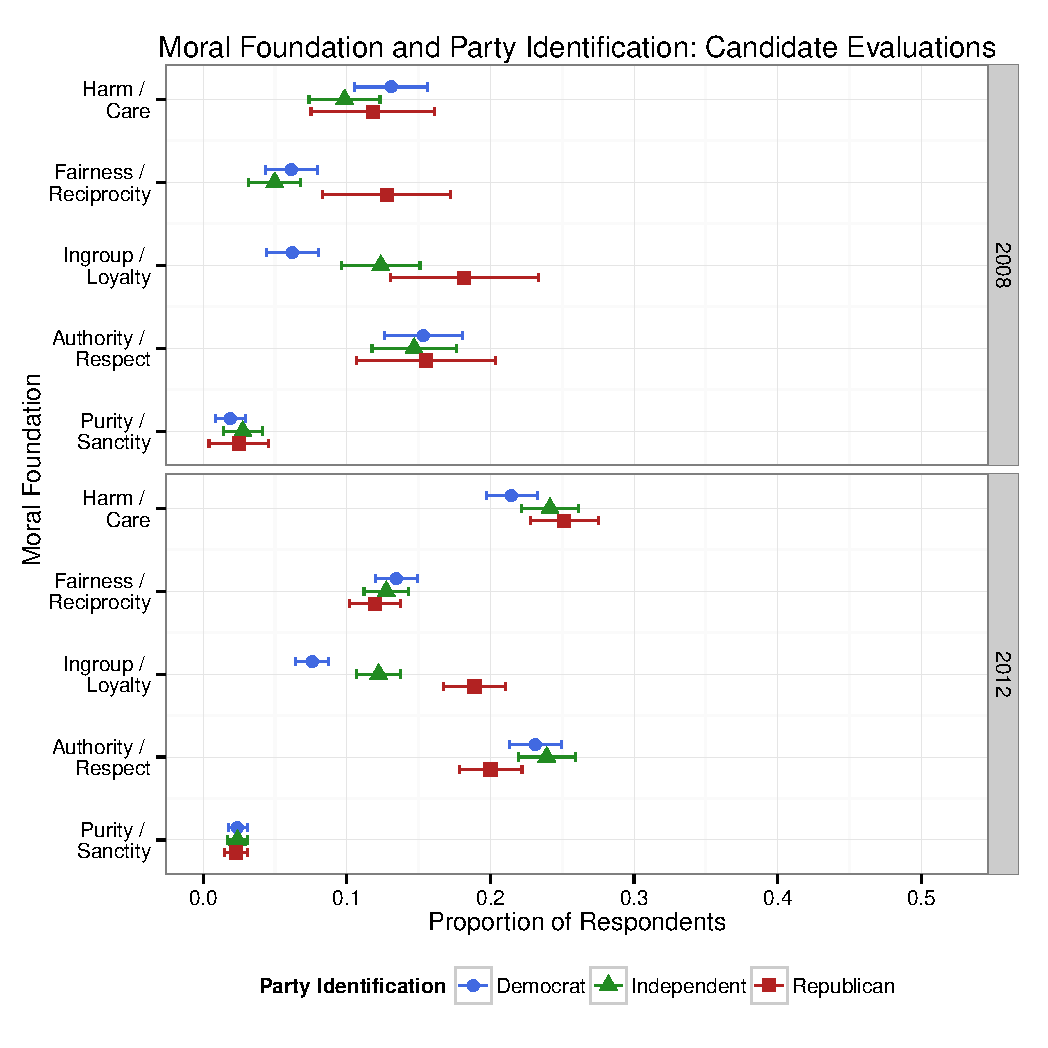
\includegraphics[scale=.4]{../calc/fig/a2_mft_pid_ca.pdf}
\caption{Moral foundations and partisanship (candidate evaluations)}\label{fig:a2_mft_pid_ca}
\end{figure}

\begin{figure}[ht]\centering
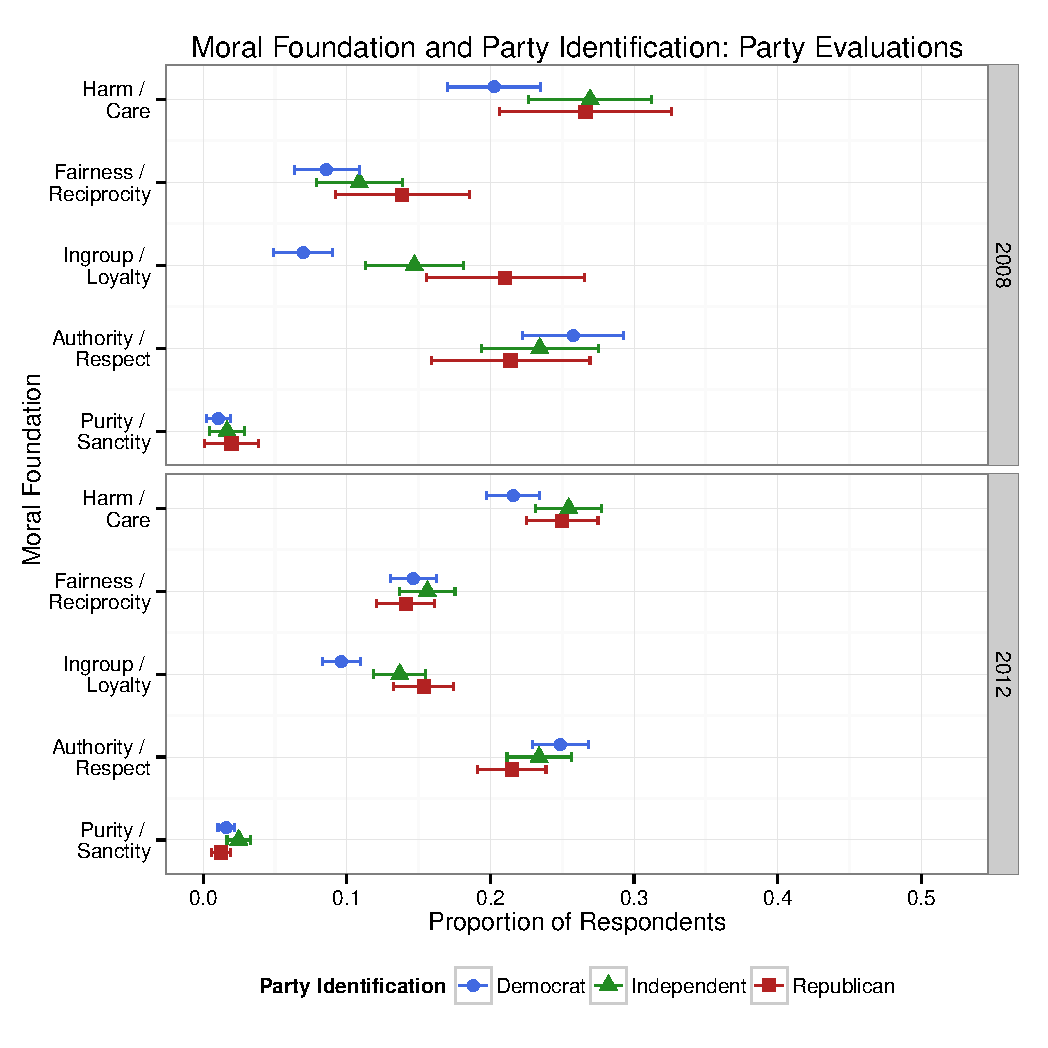
\includegraphics[scale=.4]{../calc/fig/a3_mft_pid_pa.pdf}
\caption{Moral foundations and partisanship (party evaluations)}\label{fig:a3_mft_pid_pa}
\end{figure}


\clearpage
\section{Tables of Logit Model Estimates}\label{app:models}
\renewcommand\thefigure{\thesection.\arabic{figure}}
\renewcommand\thetable{\thesection.\arabic{table}}
\setcounter{figure}{0}
\setcounter{table}{0}


% Table created by stargazer v.5.2 by Marek Hlavac, Harvard University. E-mail: hlavac at fas.harvard.edu
% Date and time: Wed, Sep 16, 2015 - 10:57:06 AM
% Requires LaTeX packages: dcolumn 
\begin{table}[ht] \centering 
  \caption{Logit Models Predicting References to four Moral Foundations using Ideology} 
  \label{tab:m1_mft} 
\tiny 
\begin{tabular}{@{\extracolsep{-15pt}}lD{.}{.}{-3} D{.}{.}{-3} D{.}{.}{-3} D{.}{.}{-3} D{.}{.}{-3} D{.}{.}{-3} D{.}{.}{-3} D{.}{.}{-3} } 
\\[-1.8ex]\hline 
\hline \\[-1.8ex] 
 & \multicolumn{8}{c}{\textit{Dependent variable:}} \\ 
\cline{2-9} 
\\[-1.8ex] & \multicolumn{2}{c}{Harm / Care} & \multicolumn{2}{c}{Fairness / Reciprocity} & \multicolumn{2}{c}{Ingroup / Loyalty} & \multicolumn{2}{c}{Authority / Respect} \\ 
 & \multicolumn{1}{c}{2008} & \multicolumn{1}{c}{2012} & \multicolumn{1}{c}{2008} & \multicolumn{1}{c}{2012} & \multicolumn{1}{c}{2008} & \multicolumn{1}{c}{2012} & \multicolumn{1}{c}{2008} & \multicolumn{1}{c}{2012} \\ 
\hline \\[-1.8ex] 
 Conservative & -0.105 & -0.327^{***} & -0.005 & -0.440^{***} & 0.288 & 0.407^{***} & -0.342^{**} & -0.308^{***} \\ 
  & (0.160) & (0.084) & (0.198) & (0.093) & (0.192) & (0.104) & (0.153) & (0.085) \\ 
  Moderate & -0.144 & -0.383^{***} & -0.280 & -0.480^{***} & 0.158 & 0.133 & -0.442^{***} & -0.129 \\ 
  & (0.165) & (0.085) & (0.217) & (0.096) & (0.202) & (0.110) & (0.159) & (0.085) \\ 
  Church Attendance & -0.025 & -0.014 & -0.015 & 0.002 & 0.052 & 0.074^{***} & 0.064^{*} & -0.026 \\ 
  & (0.039) & (0.020) & (0.048) & (0.022) & (0.044) & (0.023) & (0.037) & (0.020) \\ 
  Education (College Degree) & 0.318^{**} & 0.032 & 0.306^{*} & 0.315^{***} & 0.458^{***} & 0.138^{*} & 0.321^{**} & 0.235^{***} \\ 
  & (0.140) & (0.070) & (0.182) & (0.077) & (0.171) & (0.083) & (0.134) & (0.070) \\ 
  Age & -0.017^{***} & -0.004^{**} & 0.010^{**} & 0.003 & 0.001 & 0.002 & -0.004 & 0.008^{***} \\ 
  & (0.004) & (0.002) & (0.005) & (0.002) & (0.005) & (0.002) & (0.004) & (0.002) \\ 
  Sex (Female) & 0.074 & 0.274^{***} & 0.154 & 0.133^{*} & -0.085 & -0.007 & -0.182 & -0.069 \\ 
  & (0.129) & (0.067) & (0.164) & (0.076) & (0.152) & (0.081) & (0.124) & (0.067) \\ 
  Race (African American) & -0.044 & -0.028 & -0.102 & -0.139 & 0.235 & 0.012 & -0.071 & 0.417^{***} \\ 
  & (0.166) & (0.092) & (0.219) & (0.108) & (0.191) & (0.114) & (0.160) & (0.091) \\ 
  Number of Words & 0.013^{***} & 0.011^{***} & 0.008^{***} & 0.008^{***} & 0.011^{***} & 0.011^{***} & 0.010^{***} & 0.012^{***} \\ 
  & (0.001) & (0.001) & (0.001) & (0.0005) & (0.001) & (0.001) & (0.001) & (0.001) \\ 
  Constant & -1.193^{***} & -1.108^{***} & -3.164^{***} & -1.935^{***} & -3.062^{***} & -2.839^{***} & -1.362^{***} & -1.811^{***} \\ 
  & (0.249) & (0.126) & (0.335) & (0.144) & (0.315) & (0.163) & (0.241) & (0.132) \\ 
 \hline \\[-1.8ex] 
Observations & \multicolumn{1}{c}{1,468} & \multicolumn{1}{c}{4,691} & \multicolumn{1}{c}{1,468} & \multicolumn{1}{c}{4,691} & \multicolumn{1}{c}{1,468} & \multicolumn{1}{c}{4,691} & \multicolumn{1}{c}{1,468} & \multicolumn{1}{c}{4,691} \\ 
Log Likelihood & \multicolumn{1}{c}{-754.236} & \multicolumn{1}{c}{-2,718.587} & \multicolumn{1}{c}{-528.080} & \multicolumn{1}{c}{-2,251.633} & \multicolumn{1}{c}{-586.828} & \multicolumn{1}{c}{-2,015.282} & \multicolumn{1}{c}{-802.048} & \multicolumn{1}{c}{-2,684.276} \\ 
Akaike Inf. Crit. & \multicolumn{1}{c}{1,526.472} & \multicolumn{1}{c}{5,455.174} & \multicolumn{1}{c}{1,074.159} & \multicolumn{1}{c}{4,521.265} & \multicolumn{1}{c}{1,191.656} & \multicolumn{1}{c}{4,048.565} & \multicolumn{1}{c}{1,622.097} & \multicolumn{1}{c}{5,386.553} \\ 
\hline 
\hline \\[-1.8ex] 
\textit{Note:}  & \multicolumn{8}{r}{$^{*}$p$<$0.1; $^{**}$p$<$0.05; $^{***}$p$<$0.01} \\ 
\end{tabular} 
\end{table} 


% Table created by stargazer v.5.2 by Marek Hlavac, Harvard University. E-mail: hlavac at fas.harvard.edu
% Date and time: Tue, Nov 10, 2015 - 12:11:17 PM
% Requires LaTeX packages: dcolumn 
\begin{table}[ht] \centering 
  \caption{Logit Models Predicting Democratic Vote Choice Based on Moral Foundations} 
  \label{tab:m2_vote} 
\tiny 
\begin{tabular}{@{\extracolsep{-15pt}}lD{.}{.}{-3} D{.}{.}{-3} D{.}{.}{-3} D{.}{.}{-3} } 
\\[-1.8ex]\hline 
\hline \\[-1.8ex] 
 & \multicolumn{4}{c}{\textit{Dependent variable:}} \\ 
\cline{2-5} 
\\[-1.8ex] & \multicolumn{4}{c}{Vote for Democratic Presidential Candidate} \\ 
 & \multicolumn{2}{c}{2008} & \multicolumn{2}{c}{2012} \\ 
\\[-1.8ex] & \multicolumn{1}{c}{(1)} & \multicolumn{1}{c}{(2)} & \multicolumn{1}{c}{(3)} & \multicolumn{1}{c}{(4)}\\ 
\hline \\[-1.8ex] 
 Harm / Care & 0.292^{**} & -0.099 & 0.270^{***} & 0.286^{***} \\ 
  & (0.122) & (0.183) & (0.079) & (0.111) \\ 
  Fairness / Reciprocity & -0.207 & -0.245 & 0.376^{***} & 0.344^{***} \\ 
  & (0.167) & (0.273) & (0.090) & (0.124) \\ 
  Ingroup / Loyalty & -0.348^{**} & -0.087 & -0.481^{***} & -0.341^{***} \\ 
  & (0.140) & (0.214) & (0.086) & (0.118) \\ 
  Authority / Respect & 0.408^{***} & 0.209 & 0.507^{***} & 0.245^{**} \\ 
  & (0.132) & (0.200) & (0.081) & (0.111) \\ 
  Party Identification (Democrat) &  & 2.888^{***} &  & 2.592^{***} \\ 
  &  & (0.183) &  & (0.131) \\ 
  Party Identification (Republican) &  & -2.260^{***} &  & -2.560^{***} \\ 
  &  & (0.411) &  & (0.143) \\ 
  Church Attendance & -0.226^{***} & -0.099^{*} & -0.311^{***} & -0.274^{***} \\ 
  & (0.033) & (0.051) & (0.022) & (0.030) \\ 
  Education (College Degree) & -0.362^{***} & -0.343^{*} & 0.077 & 0.213^{**} \\ 
  & (0.121) & (0.177) & (0.079) & (0.108) \\ 
  Age & -0.017^{***} & -0.030^{***} & -0.014^{***} & -0.022^{***} \\ 
  & (0.003) & (0.005) & (0.002) & (0.003) \\ 
  Sex (Female) & 0.388^{***} & 0.101 & 0.365^{***} & 0.306^{***} \\ 
  & (0.117) & (0.172) & (0.075) & (0.103) \\ 
  Race (African American) & 4.330^{***} & 3.693^{***} & 3.974^{***} & 3.056^{***} \\ 
  & (0.390) & (0.468) & (0.229) & (0.256) \\ 
  Constant & 1.269^{***} & 0.592^{**} & 0.743^{***} & 1.007^{***} \\ 
  & (0.207) & (0.291) & (0.136) & (0.190) \\ 
 \hline \\[-1.8ex] 
Observations & \multicolumn{1}{c}{1,822} & \multicolumn{1}{c}{1,313} & \multicolumn{1}{c}{3,973} & \multicolumn{1}{c}{3,963} \\ 
Log Likelihood & \multicolumn{1}{c}{-886.197} & \multicolumn{1}{c}{-453.056} & \multicolumn{1}{c}{-2,096.122} & \multicolumn{1}{c}{-1,237.334} \\ 
Akaike Inf. Crit. & \multicolumn{1}{c}{1,792.393} & \multicolumn{1}{c}{930.112} & \multicolumn{1}{c}{4,212.244} & \multicolumn{1}{c}{2,498.669} \\ 
\hline 
\hline \\[-1.8ex] 
\textit{Note:}  & \multicolumn{4}{r}{$^{*}$p$<$0.1; $^{**}$p$<$0.05; $^{***}$p$<$0.01} \\ 
\end{tabular} 
\end{table} 


% Table created by stargazer v.5.1 by Marek Hlavac, Harvard University. E-mail: hlavac at fas.harvard.edu
% Date and time: Sun, Dec 14, 2014 - 03:16:26 PM
% Requires LaTeX packages: dcolumn 
\begin{table}[ht] \centering 
  \caption{Logit Models Predicting Overall References to Moral Foundations} 
  \label{tab:m3_learn} 
\tiny 
\begin{tabular}{@{\extracolsep{-15pt}}lD{.}{.}{-3} D{.}{.}{-3} D{.}{.}{-3} D{.}{.}{-3} D{.}{.}{-3} D{.}{.}{-3} D{.}{.}{-3} D{.}{.}{-3} } 
\\[-1.8ex]\hline 
\hline \\[-1.8ex] 
 & \multicolumn{8}{c}{\textit{Dependent variable:}} \\ 
\cline{2-9} 
\\[-1.8ex] & \multicolumn{8}{c}{Reference to any Moral Foundation} \\ 
 & \multicolumn{1}{c}{2008} & \multicolumn{1}{c}{2012} & \multicolumn{1}{c}{2008} & \multicolumn{1}{c}{2012} & \multicolumn{1}{c}{2008} & \multicolumn{1}{c}{2012} & \multicolumn{1}{c}{2008} & \multicolumn{1}{c}{2012} \\ 
\\[-1.8ex] & \multicolumn{1}{c}{(1)} & \multicolumn{1}{c}{(2)} & \multicolumn{1}{c}{(3)} & \multicolumn{1}{c}{(4)} & \multicolumn{1}{c}{(5)} & \multicolumn{1}{c}{(6)} & \multicolumn{1}{c}{(7)} & \multicolumn{1}{c}{(8)}\\ 
\hline \\[-1.8ex] 
 Political Knowledge & 0.261^{**} & 0.149^{***} &  &  &  &  & 0.219^{*} & 0.142^{***} \\ 
  & (0.117) & (0.033) &  &  &  &  & (0.125) & (0.035) \\ 
  Political Media Exposure &  &  & 0.027^{***} & 0.019^{***} &  &  & 0.017^{*} & 0.011^{*} \\ 
  &  &  & (0.009) & (0.006) &  &  & (0.010) & (0.006) \\ 
  Political Discussions &  &  &  &  & 0.001 & 0.091^{***} & -0.011 & 0.079^{***} \\ 
  &  &  &  &  & (0.025) & (0.019) & (0.026) & (0.019) \\ 
  Church Attendance & 0.022 & -0.020 & 0.022 & -0.020 & 0.013 & -0.018 & 0.012 & -0.019 \\ 
  & (0.031) & (0.019) & (0.030) & (0.019) & (0.033) & (0.020) & (0.033) & (0.020) \\ 
  Education (College Degree) & 0.379^{***} & 0.185^{**} & 0.442^{***} & 0.239^{***} & 0.480^{***} & 0.282^{***} & 0.402^{***} & 0.183^{**} \\ 
  & (0.114) & (0.077) & (0.106) & (0.075) & (0.116) & (0.077) & (0.121) & (0.081) \\ 
  Age & -0.005 & -0.002 & -0.008^{**} & -0.003 & -0.003 & 0.0002 & -0.004 & -0.003 \\ 
  & (0.003) & (0.002) & (0.003) & (0.002) & (0.003) & (0.002) & (0.004) & (0.002) \\ 
  Sex (Female) & -0.094 & 0.226^{***} & -0.064 & 0.204^{***} & -0.135 & 0.195^{***} & -0.123 & 0.243^{***} \\ 
  & (0.109) & (0.068) & (0.104) & (0.067) & (0.114) & (0.069) & (0.115) & (0.071) \\ 
  Race (African American) & -0.057 & 0.445^{***} & -0.096 & 0.367^{***} & -0.070 & 0.358^{***} & -0.023 & 0.418^{***} \\ 
  & (0.127) & (0.091) & (0.118) & (0.088) & (0.133) & (0.092) & (0.135) & (0.094) \\ 
  Number of Words & 0.029^{***} & 0.025^{***} & 0.029^{***} & 0.026^{***} & 0.028^{***} & 0.025^{***} & 0.027^{***} & 0.025^{***} \\ 
  & (0.002) & (0.001) & (0.002) & (0.001) & (0.002) & (0.001) & (0.002) & (0.001) \\ 
  Constant & -1.411^{***} & -1.319^{***} & -1.481^{***} & -1.067^{***} & -1.274^{***} & -1.066^{***} & -1.484^{***} & -1.464^{***} \\ 
  & (0.201) & (0.143) & (0.195) & (0.122) & (0.209) & (0.124) & (0.227) & (0.152) \\ 
 \hline \\[-1.8ex] 
Observations & \multicolumn{1}{c}{1,845} & \multicolumn{1}{c}{5,147} & \multicolumn{1}{c}{2,031} & \multicolumn{1}{c}{5,177} & \multicolumn{1}{c}{1,648} & \multicolumn{1}{c}{4,842} & \multicolumn{1}{c}{1,646} & \multicolumn{1}{c}{4,807} \\ 
Log Likelihood & \multicolumn{1}{c}{-1,016.596} & \multicolumn{1}{c}{-2,670.308} & \multicolumn{1}{c}{-1,118.869} & \multicolumn{1}{c}{-2,689.725} & \multicolumn{1}{c}{-915.937} & \multicolumn{1}{c}{-2,495.047} & \multicolumn{1}{c}{-912.088} & \multicolumn{1}{c}{-2,467.724} \\ 
Akaike Inf. Crit. & \multicolumn{1}{c}{2,049.192} & \multicolumn{1}{c}{5,356.616} & \multicolumn{1}{c}{2,253.737} & \multicolumn{1}{c}{5,395.450} & \multicolumn{1}{c}{1,847.874} & \multicolumn{1}{c}{5,006.093} & \multicolumn{1}{c}{1,844.175} & \multicolumn{1}{c}{4,955.448} \\ 
\hline 
\hline \\[-1.8ex] 
\textit{Note:}  & \multicolumn{8}{r}{$^{*}$p$<$0.1; $^{**}$p$<$0.05; $^{***}$p$<$0.01} \\ 
\end{tabular} 
\end{table} 



\clearpage
\section{Alternative Model Specifications and Robustness Checks}\label{app:robust}
\renewcommand\thefigure{\thesection.\arabic{figure}}
\renewcommand\thetable{\thesection.\arabic{table}}
\setcounter{figure}{0}
\setcounter{table}{0}

\begin{figure}[ht]\centering
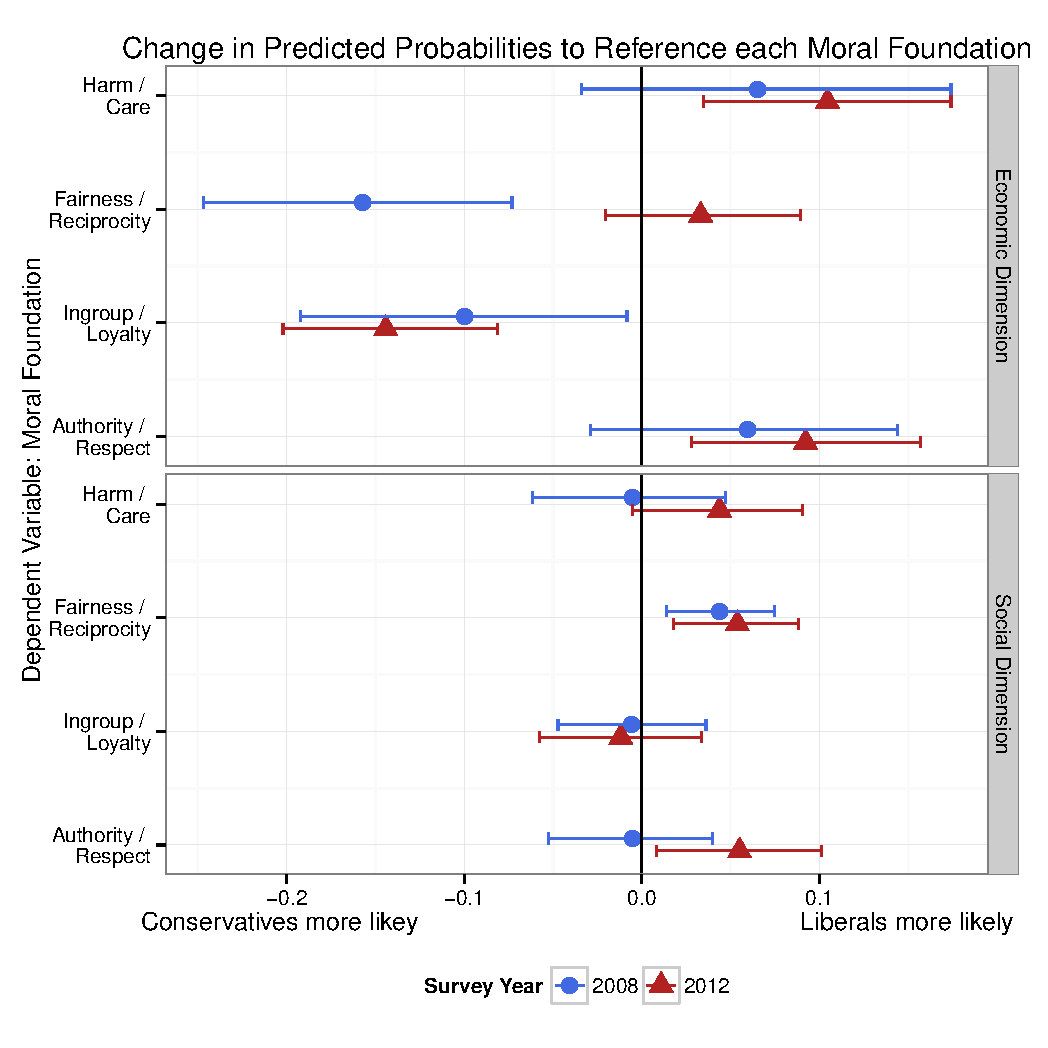
\includegraphics[scale=.4]{../calc/fig/m1b_mft.pdf}
\caption{Difference in predicted probabilities to reference each moral foundation between liberals and conservatives on economic and social dimension}\label{fig:m1b_mft}
\end{figure}

\begin{figure}\centering
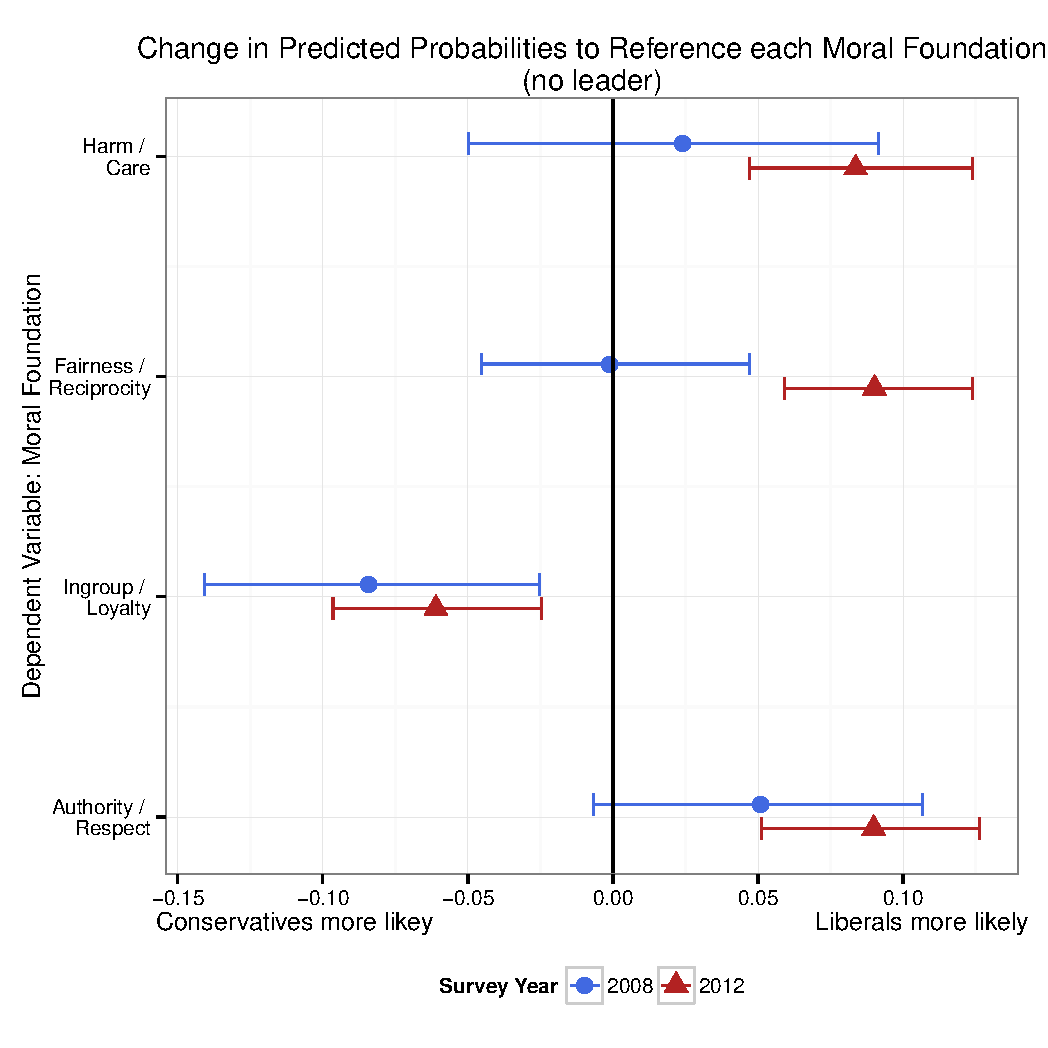
\includegraphics[scale=.4]{../calc/fig/m1_mft_noleader.pdf}
\caption{Difference in predicted probabilities to reference each moral foundation between liberals and conservatives (omitting ``leader'' from the dictionary)}\label{fig:m1_mft_noleader}
\end{figure}

\begin{figure}\centering
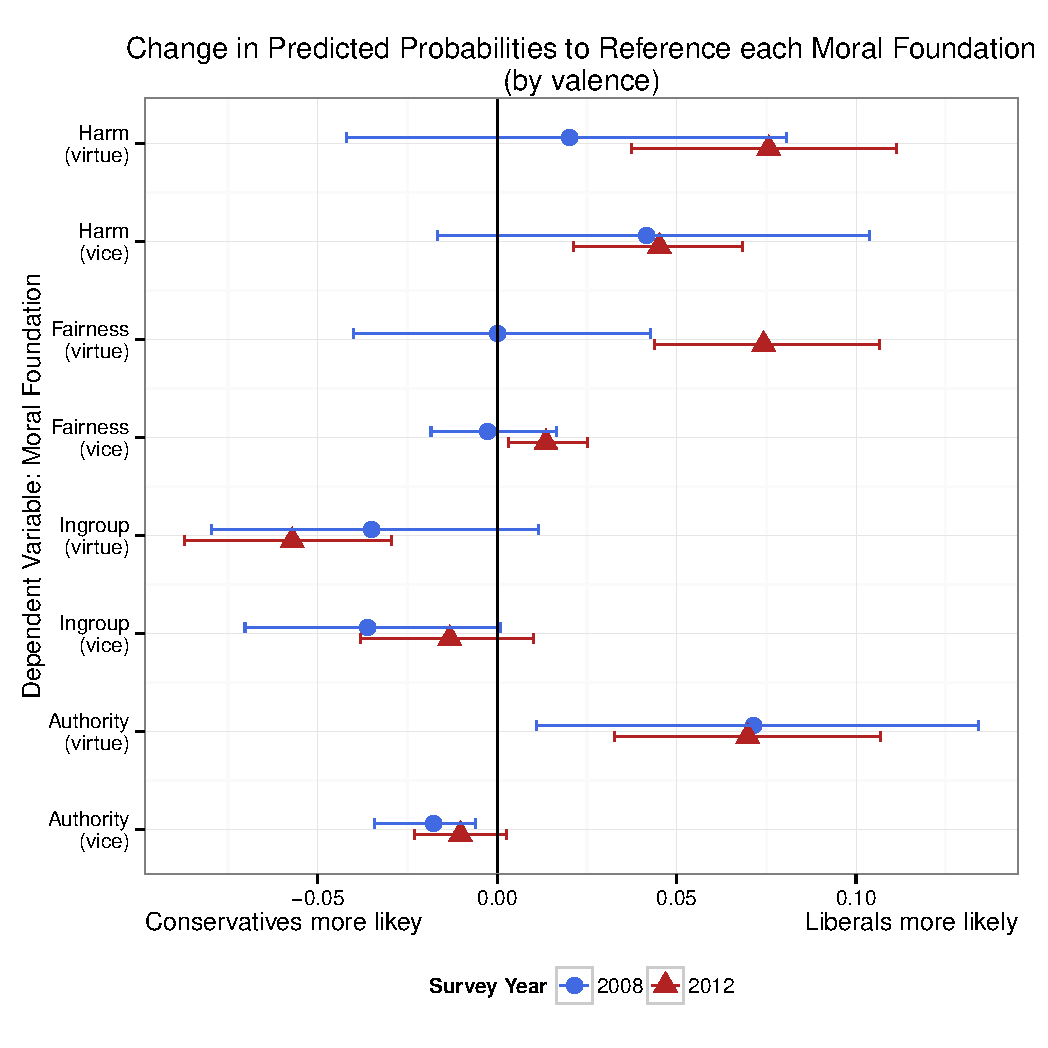
\includegraphics[scale=.4]{../calc/fig/m1c_mft.pdf}
\caption{Difference in predicted probabilities to reference each moral foundation between liberals and conservatives (dis-aggregating moral foundations by valence)}\label{fig:m1c_mft}
\end{figure}

\begin{figure}\centering
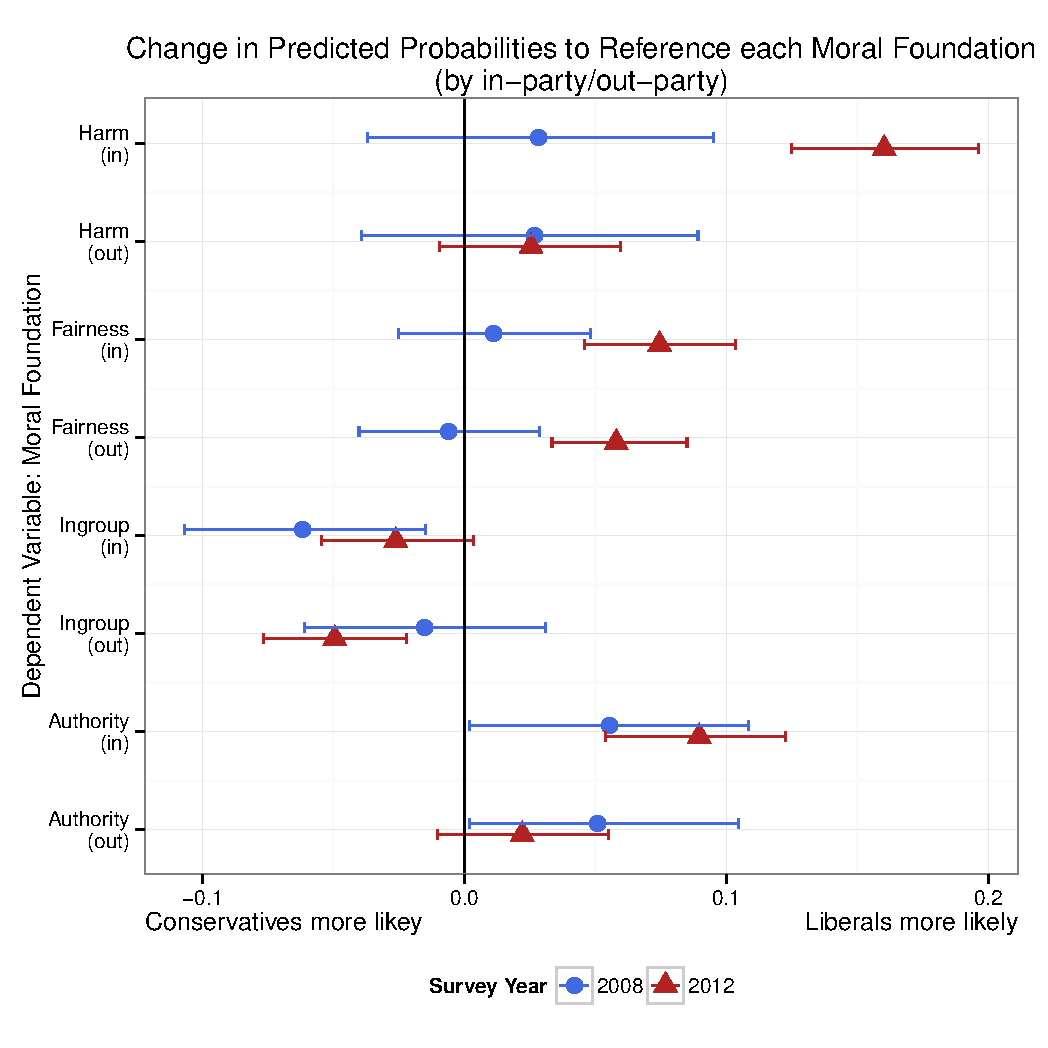
\includegraphics[scale=.4]{../calc/fig/m1d_mft.pdf}
\caption{Difference in predicted probabilities to reference each moral foundation between liberals and conservatives (dis-aggregating statements by in- and out-party)}\label{fig:m1d_mft}
\end{figure}

\begin{figure}\centering
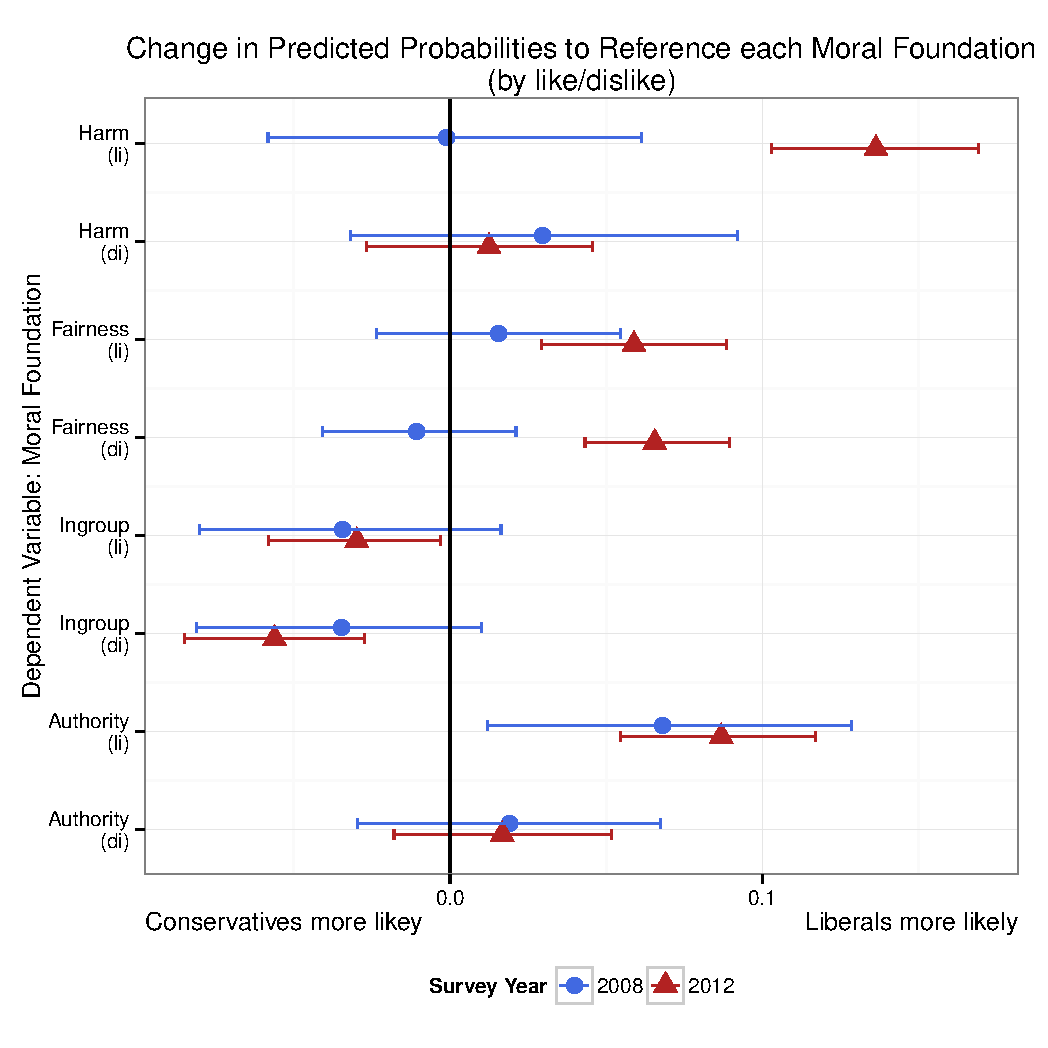
\includegraphics[scale=.4]{../calc/fig/m1e_mft.pdf}
\caption{Difference in predicted probabilities to reference each moral foundation between liberals and conservatives (dis-aggregating statements by likes and dislikes)}\label{fig:m1e_mft}
\end{figure}

\end{document}